\documentclass[12pt, a4paper, openany]{book}
\usepackage{../generalStyle}

\graphicspath{ {./chapters_ulerich/img/} }

\lstset{
  language=Java,
  basicstyle=\ttfamily,
  keywordstyle=\color{blue},
  stringstyle=\color{red},
  commentstyle=\color{orange},
  morecomment=[l][\color{magenta}]{\#}
}

\begin{document}

\title{Analisi e Progetto di Algoritmi}

\author{
    Elia Ronchetti\\
	\small{\href{https://t.me/ulerich}{@ulerich}}
}

\date{2023/2024}

\maketitle

\tableofcontents
\chapter{Programmazione Dinamica}
\section{Introduzione}
\paragraph{La programmazione dinamica} è una tecnica di programmazione che viene utilizzata per risolvere problemi più velocemente rispetto ad una soluzione ricorsiva a discapito di un maggiore consumo di memoria.
\\Viene tipicamente applicata a \emph{problemi di ottimizzazione}. Questi problemi ammettono (in genere) molte soluzioni possibili, ciascuna con un valore, di cui ci interessa trovare quella con il valore ottimo (massimo o minimo) che chiameremo \emph{soluzione ottimale}.

\paragraph{Approccio generale}
La programmazione dinamica risolve un problema combinando le soluzioni dei suoi sottoproblemi.\\
l'approccio generale si può riassumere in 4 passi:
\begin{enumerate}
	\item Caratterizzare la struttura di una soluzione ottimale.
	\item Definire ricorsivamente il valore di una soluzione ottimale (e quindi di tutte).
	\item Calcolare il valore delle soluzinoi ottimali, tipicamente in maniera bottom-up,
	      memorizzando i loro valori in tabelle.
	\item Costruire una soluzione ottimale usando le informazioni già calcolate e memorizzate.
\end{enumerate}

\paragraph{Proprietà necessarie} per applicare la porgrammazione dinamica in modo utile ed efficiente:
\begin{enumerate}
	\item \textbf{Sottostruttura ottima} :Una soluzione ottima è esprimibile in termini di soluzioni ottime di sottoproblemi
	\item \textbf{Sovrapposizione dei sottoproblemi}: L'insieme dei sottoproblemi distinti ha cardinalità di molto inferiore all'insieme delle soluzioni possibili da cui vogliamo seleziona quella ottima. Quindi un problema deve apparire molte volte come sottoproblema di altri problemi
\end{enumerate}

\paragraph{DP vs D-et-I}
Come il metodo divide-et-impera, la programmazione dinamica risolve un problema combinando le soluzioni dei suoi sottoproblemi.\\
La programmazione dinamica è utile quando i sottoproblemi si sovrappongono, ovvero \emph{diversi sottoproblemi contengono gli stessi sottoproblemi}\\
D-et-I risolverebbe inutilmente i sottoproblemi ogni volta, mentre un algoritmo di programmazione dinamica risolve ogni sottoproblema una sola volta e ne memorizza la soluzione in una tabella, in modo da evitare di dover ripetere ogni volta il calcolo della soluzione di un sottoproblema già risolto.
\subparagraph{Esempio: Fibonacci}
Calcolando il numero di Fibonacci, se utilizziamo la tecnica D-et-I l'albero delle chiamate ricorsive \emph{esplode}.
Se invece utilizzando la programmazione dinamica memorizziamo i valori già calcolati possiamo evitare di ripetere inutilmente calcoli già risolti.

\section{Weighted Interval Scheduling}
\paragraph{Introduzione}Il problema dello scheduling di attività riguarda la gestione di un insime di attività caratterizzate da un tempo di inizio, un tempo di fine e un valore.
L'obiettivo è quello di determinare un insieme di attività mutualmente compatibili il cui valore totale è massimo.

Un insieme di attività si dice\emph{ mutualmente compatibili} se per ogni attività di tale insieme, nessun'altra attività dell'insieme si sovrappone a questa.


\paragraph{Pseudocodice}
$p(i)$ è il più grande indice i > j tale che l'intervallo di indice i non si sovrappone all'intervallo di indice j.
\begin{lstlisting}
WIS
	M[0] = 0
	for i = 1 to n
		M[i] = max(v$_i$ + M[p(i)], M[i-1])
\end{lstlisting}
In pratica, essendo OPT la soluzione ottimale, il valore di M[i] è:
\begin{itemize}
	\item $v_i$ = $M[p(i)]$ se $i \in OPT$
	\item $M[i-1]$ se $i \notin OPT$
\end{itemize}

\section{Knapsack Problem 0/1}
\paragraph{il problema} Ci sono n oggetti ai quali sono associati un peso e un valore. Ho uno zaino di capictà in peso C. L'obiettivo è prendere k oggetti tali per cui il valore sia massimo senza superare la capacità dello zaino.\\
Questo tipo di problema si chiama \emph{0/1} perchè un oggetto \emph{O lo prendo tutto o non lo prendo proprio}. Si utilizza questa terminologia per differenziare lo 0/1 dal Knapsack Frazionario che vedremo in seguito.
\paragraph{Input} $I = \{e_1,...,e_n\} \forall  i, e_i$ ha associati due valori: $v_i$ (valore) e $w_i$ (peso). W = Peso totale dello zaino.
\paragraph{Output} Trovare un sottoinsieme $ S \subset I $ di elementi $S = \{e_{j,1}, ..., e_{j,k}\} , 1 \leq j_l \leq n$ tc. soddisfa 2 vincoli:
\begin{itemize}
	\item max$(\Sigma_{e_i \in S}V_i)$ ;
	\item $\Sigma_{e_i \in S} W_i \leq W$.
\end{itemize}

\paragraph{Sottostruttura ottima}
La sottostruttura ottima del problema non è molto straight-forward. facciamo un esempio:
\subparagraph*{}Se abbiamo un problema (che non necessariamente ci interessa definire) la cui soluzione S è $\{e_2,e_3,e_4\}$.\\
Se eliminiamo l'elemento $e_i$, S è comunque la soluzione ottimale dell'input I (senza considerare $e_i$)? No, perche se nell'input esisteva un altro elemento con lo stesso peso e valore di $e_i$ che non era stato considerato per mancanza di spazio, allora la solzione ottimale è diversa.
\\Bisogna quindi aggiungere il vincolo che gli elementi sono ordinati e la soluzione è espressa in funzione dell'ordine degli elementi

\section{LCS}
LCS, o Longest Common Susbequence è un problema di programmazione dinamica in cui si richiede di trovare la più grande sottosequenza comune a due sottosequenze.

\paragraph{Definizione del problema}
Date due sequenze $X$ e $Y$, trovare \emph{la più lunga sottosequenza comune di caratteri} (non necessariamente consecutivi).\\
Una sottosequenza di una data sequenza è la sequenza stessa alla quale sono stati tolti zero o più elementi.
Una sottosequenza comune di due sequenze è una sottosequenza di entrambe.
\\Il problema della LCS può essere risolto in modo efficiente applicando la programmazione dinamica.

\subsection*{Sottostruttura ottima di una LCS}
LCS gode della proprietà della sottostruttura ottima, infatti:
\\Data una sequenza $X=\{x_1,x_2,...,x_m\}$ definiamo $X_i=\{x_1,x_2,...,x_i\}$ l'i-esimo prefisso di X per $i = 0,...,m$
\paragraph{Teorema}
Siano $X=\{x_1,x_2,...,x_m\}$ e $Y=\{y_1,y_2,...,y_n\}$ le sequenze; sia $Z=\{z_1,z_2,...,z_m\}$ una qualsiasi LCS di X e Y.
\begin{enumerate}
	\item Se $x_m = y_n$, allora $z_k = x_m =y_n$ e $Z_{k-1}$ è  una LCS di $X_{m-1}$ e $Y_{n-1}$
	\item Se $x_m \neq y_n$, allora $z_k \neq x_m$ implica che Z è una LCS di $X_{m-1}$ e $Y$
	\item Se $x_m \neq y_n$, allora $z_k \neq y_n$ implica che Z è una LCS di $X$ e $Y_{n-1}$
\end{enumerate}
La caratterizzazione di questo teorema dimostra che una LCS di due sequenze contiene al suo interno una LCS di prefissi delle due sequenze.
Quindi il problema della più lunga sottosequenza comune gode della proprietà della sottostruttura ottima

\spiegazione{
	Se sappiamo che \emph{Z è una (qualsiasi) LCS di X e Y}, allora se ne deduce che:
	\\(1) Se gli ultimi elementi di X e Y sono uguali, allora è anche l'ultimo elemento di Z. Inoltre implica che $Z_{k-1}$, quindi Z se togliamo il suo ultimo elemento, è una LCS di X e Y a cui sono stati tolti l'ultimo elemento ciascuno.
	\\Se gli ultimi elementi di X e Y NON sono uguali invece, qui ci sono due opzioni: (2) o l'ultimo elemento di Z è uguale all'ultimo elemento di Y, in tal caso Z è una lcs di Y e X senza l'ultimo elemento, oppure (3) viceversa
}
\paragraph{La soluzione ricorsiva}
Definiamo $c[i,j]$ come la lunghezza di una LCS delle sequenze $X_i$ e $Y_j$
\begin{equation*}
	c[i,j] = \begin{cases}
		0                       & \text{se $i = 0$ o $j = 0$} \\
		c[i-1,j-1] + 1          & \text{se $x_i = y_j$}       \\
		max(c[i,j-1], c[i-1,j]) & \text{se $x_i \neq y_j$}
	\end{cases}
\end{equation*}

\paragraph{pseudocodice}
\begin{lstlisting}
def LCS-LENGHT(X,Y):
	m = X.lenght
	n = Y.lenght
	b[1..m,1..n] e c[0..m,0..m] -> nuove tabelle
	for i = 1 to m
		c[i,0] = 0
	for j= 0 to n
		c[0,j] = 0
	for i = 1 to m
		for j = 1 to n
			if $x_i$ == $y_i$
				c[i,j] = c[i-1,j-1] + 1  
				b[i,j] = $\nwarrow $
			elif c[i - 1,j] $\geq$ c[i,j-1]
				c[i,j] = c[i-1,j]  
				b[i,j] = $\uparrow $
			else
				c[i,j] = c[i,j-1]  
				b[i,j] = $\leftarrow $
	return c e b
\end{lstlisting}



\subsection*{Esercizio: LCS $\geq L$}

\paragraph*{Istanza} Date due sequenze:\\
$X = <x_1,...,x_m>$ di lunghezza $m$\\
$Y = <y_1,...,y_n>$ di lunghezza $n$\\
e dato un $L \geq 0$ stabilire se \emph{La lunghezza di una qualunque LCS di $X$ e $Y$ è $\geq L$}.
\\Quindi TRUE sse $\exists$ una LCS(X,Y) di lunghezza $geq L$

\paragraph*{Istanza di un qualunque sottoproblema}
\begin{itemize}
	\item[] $X_i$ (con $0 \leq i \leq m$)
	\item[] $Y_j$ (con $0 \leq j \leq n$)
	\item[] $l$ (con $0 \leq l \leq L$)
\end{itemize}
Quindi ogni sottoproblema è individuato da una n-pla (i, j, l) con $0 \leq i \leq m$, $0 \leq j \leq n$, $0 \leq l \leq L$.
La soluzione di ogni sottoproblema sarà un valore \emph{True/False} a se cibda cge esusta i nebi yba LCS di $X_i$ e $Y_j$ di lunghezza $geq l$.
Pertanto introduciamo una variabile per ogni sottoproblema destinata a contenerne la soluzione.
\paragraph*{Definizione delle Variabiili}
$\forall i\in \{0,...,m\}, \forall j\in\{0,...n\}, \forall l\in \{0...,L\}$
$C_{ijl}$ è definita come soluzione del sottoproblema (i,j,l), ossia vale True sse la lunghezza di una qualunque LCS di $X_i$ e $Y_j$ è $\geq l$.
Per ogni i,j,l come sopra dobbiamo ora calcoalre il valore di $c_{ijl}$.
\paragraph*{Caso Base}
\begin{equation}
	c_{ijl} = \begin{cases}
		\text{True}  & \text{se $l = 0$}                     \\
		\text{False} & \text{se $l>0 \wedge (i<l \vee j<l)$}
	\end{cases}
\end{equation}
\spiegazione{
	Se $l=0$ c.. è truè perchè ovviamente qualunque LCS è maggiore o uguale a 0.\\
	Se invece $l>0$, ma una delle due stringhe è minore di $l$ allora automaticamente non può esistere una LCS più lunga di $l$
}
\paragraph*{Passo Ricorsivo}
Comprende tute le tuple (i,j,l) con $l>0 \wedge i\geq l \wedge j \geq l$
\begin{itemize}
	\item[Caso 1] sse $x_i = y_j$\\ $c_{ijl} = c_{i-1,j-1,l-1}$ %Non c'è il +1 perchè è True/False pirla%
	\item[Casi 2] se  $x_i \neq y_j$,
		\begin{itemize}
			\item[2a] LCS($X_i,Y_j$) termina con $z_k \neq x_i$ \\ $c_{i-1,j,l}$
			\item[2b] LCS($X_i,Y_j$) termina con $z_k \neq y_j$ \\ $c_{i,j-1,l}$
		\end{itemize}
\end{itemize}
Risolvendo $\exists$ una LCS($X_i,Y_j$) di lunghezza $\geq l$ sse ciò si verifica in almeno uno dei due casi, per cui:
$c_{ijl} = c_{i-1,j,l} \vee c_{i,j-1,l}$.
Riassumendo, il passo ricorsivo è:
Dati $l>0 \wedge i\geq l \wedge j \geq l$
\begin{equation}
	C_{ijl} = \begin{cases}
		C_{i-1,j-1,l-1}              & x_i = y_j    \\
		C_{i-1,j,l} \vee C_{i,j-1,l} & x_i \neq y_j
	\end{cases}
\end{equation}

\spiegazione{
	Siccome si tratta di programmazione dinamica, e siccome tutti i valori che abbiamo calcolato vengono salvati in una matrice (C)
	prendo il valore di quella matrice, già inizializzata con il caso base, che più si "addice al caso"}

\paragraph*{Soluzione}
Con istanza X,Y,L la soluzione del problema è il valore di $c_{m,n,L}$

\paragraph*{Pseudocodice} LCS $\geq$ L
\begin{lstlisting}[style=small]
def LCS-MAGGIORE-L(X,Y,L)
	m = lenght[X]
	n = lenght[Y]
	for i=0 to m
		for j=0 to n
			c$_{i,j,0}$ = True
	for l=1 to L
		for i=0 to m
			for j=0 to n
				if i < l $\vee$ j < l
					c$_{i,j,l}$ = False
				elif x$_i$ = y$_j$
					c$_{i,j,l}$ = c$_{i-1,j-1,l-1}$
				elif x$_i$ \neq y$_j$
					c$_{i,j,l}$ = c$_{i-1,j,l}$ $\vee$ c$_{i,j-1,l}$
	return c$_{m,n,L}$
\end{lstlisting}

\section{LIS}
LIS, o Longest Increasing Subsequence è un algoritmo che calcola la lunghezza della più lunga sottosequenza crescente di una determinata sequenza.
A differenza di LCS, LIS viene calcolata su una sola sequenza, in questo caso una sottosequenza è un qualunque sequenza di caratteri che fanno parte della nostra sequenza.

\paragraph*{Definizione del Problema}
Data una sequenza $X$ di $n$ caratteri, si vuole trovare la lunghezza della più lunga sottosequenza di caratteri \emph{strettamente crescenti} (in ordine lessicografico).
\\\textbf{Istanza:} $X=<x_1,...,x_n>$, \textbf{Soluzione:} La più lunga sotto sequenza di $X$ strettamente crescente.


\subsection*{Sottoproblema} Il sottoproblema di taglia $i$ è la più lunga sottosequenza strettamente crescente che termini con l'\emph{i-esimo} carattere di $X$.
\\Nel caso di $i=1$, la soluzione è ovviamente $1$, siccome ogni sottosequenza di dimensione 1 è strettamente crescente (e decrescente).
Mentre per i sottoproblemi di taglia maggiore di 1, ipotizzando di aver già risolto i sottoproblemi più piccoli ci basta vedere quale sia la massima lunghezza di una LIS compatibile con li carattere $x_i$ (ovvero che sia abbia l'ultimo carattere minore di $x_i$)
e aggiungerci 1.

\paragraph{Definizione delle variabili}
Definiaimo $S[i]$ come la soluzione al sottopbroblema di taglia $i$, ovvero come la lunghezza della 
più lunga sottosequenza strettamente crescente che \emph{termini} con l'i-esimo carattere di $X$

\subsection*{Equazioni di ricorrenza}
\paragraph*{Caso Base} con $i=1$,
 $$S[i]=\begin{cases}
	 1
 \end{cases}$$
visto che è la lunghezza massima di una sottosequenza di dimensione 1.
\paragraph*{Passo Ricorsivo} con $1<i\leq n$,
$$
S[i] = \begin{cases}
	1+\text{max}\{S[j]\} | 0 \leq j < i | x_j < x_i
\end{cases}
$$
Ovvero, la soluzione è la più grande tra le soluzioni precedenti in cui l'ultimo carattere è minore del carattere $i$ aumentata di uno.
\subsection*{Soluzione}
la soluzione di LIS è il max$\{S[i]| 0 < i \leq n\}$.
\\A differenza di LCS, in LIS la soluzione non sarà mai allo stesso posto ma alla posizione del carattere in cui termina la sottosequenza più grande.
\subsection*{Pseudocodice}
\begin{lstlisting}
	def LIS(X):
		S[1] = 1
		for i = 2 to n
			max = 0
			for j = 0 to i
				if S[j] > max AND X[j] < X[i]
					max = S[j]
			S[i] = max + 1
		return max(S) 

\end{lstlisting}

\subsection*{Tempo e Spazio}
Il tempo dell'algoritmo è pari a $\Theta(n^2)$
\\Lo spazio è pari a $\Theta(n)$

\paragraph*{Per ricostruire la sequenza} potremmo ripercorrere l'array $S$ all'indietro controllando,
ogni volta che troviamo un valore minore di quello analizzato se il carattere nella posizione di tale valore sia compatibile con quello nella posizione che stiamo analizzando.


\section{LGCS / LICS} %Pagina 24 degli appunti pdf che ho preso da Elearning
LGCS, o Longest Growing Common Subsequence (LICS - Longest Increasing Common Subsequence), è una variazione di LCS in cui si richiede
di trovare la più lunga sottosequenza comune di caratteri \emph{strettamente crescenti} (in ordine alfabetico).

\paragraph*{Definizione del Problema}
Date due sequenze $X$ e $Y$, rispettivamente di $m$ ed $n$ caratteri, trovare \emph{la lunghezza della più lunga sottosequenza comune di caratteri strettamente crescenti}

\subsection*{Sottoproblema}
Il sottoproblema non prende in considerazione l'intero input, ma solo i prefissi di $X$ e $Y$ rispettivamente di dimensione $i$ e $j$.
è così definito:
\\Date due sequenze X e Y, si determini la lunghezza di una tra le più lunghe sottosequenze crescenti comuni al prefisso $X_i$ e $Y_j$.
\\Ad ogni sottoproblema è associata una \textbf{variabile} $c_{i,j}$ così definita:
\\$c_{i,j}$ = lunghezza di una tra le più lunghe sottosequenze crescenti comuni a $X_i$ e $Y_j$
\\Il problema così definito però non è risolvibile perchè \emph{manca dell'informazione}, bisogna quindi definire un problema ausiliario nel quale introdurre l'informazione mancante necessaria.

\subsection*{Problema ausiliario}
Il problema ausiliario, che ci serve a fornire le informazioni mancanti per risolvere il problema originale, è definito come segue:

\paragraph*{Definizione di Problema Ausiliario}
Date due sequenze X e Y, la soluzione è data dalla lunghezza della più lunga sottosequenza comune crescente \emph{che termini con $x_n =y_m$}.

\spiegazione{
	Viene aggiunto il vincolo che l'ultimo elemento della Soluzione sia l'ultimo elemento delle stringhe \emph{solo nel caso in cui coincidano}.
	Se questi non coincidono, la soluzione è la sequenza vuota.
	Questa richiesta, quando applicata ai sottoproblemi ci permetterà di sapere qual'è l'ultimo elemento di un sottoproblema.
}

\paragraph*{Sottoproblema} date due sequenze $X$ e $Y$ , rispettivamente di $m$ ed $n$ caratteri, si determini la lunghezza di una tra le più lunghe sottosequenze crescenti comuni
a $X_i$ e a $Y_j$ e che termina con $x_i$ e $y_j$ solo se questi coincidono.
\\ad ogni sottoproblema è associata la varaible $c_{i,j}$ così definita:
\\ $c_{i,j}$ = lunghezza di una tra le più lunghe sottosequenze crescenti comuni a $X_i$ e $Y_j$ e che termina con $x_i$ e $y_j$ solo se questi coincidono.

\spiegazione{
	Si noti quindi che per un qualunque sottoproblema di dimensione $(s, t)$, solo imponendo che la soluzione $c_{s,t}$ si riferisca ad una sottosequenza crescente comune
	a $X_s$ e $Y_t$ che termina con $x_s = y_t$ è possibile stabilire se un altro elemento $x_u = y_v$ con $u > s$ e $v > t$ possa essere accodato a tale sottosequenza (andando
	a verificare che $x_s = y_t < x_u = y_v$).
}

\subsection*{Equazioni di ricorrenza}
\paragraph*{Nota bene} %dopo spostare in teoria TODO
un equazione di ricorrenza è composta da:
\begin{itemize}
	\item Un caso base che definisce i casi più semplici che possono essere subito risolti senza ricorrere alle soluzioni dei sottoproblemi più piccoli
	\item Un passo ricorsivo che definisce come risolvere i casi più complessi a partire dalle soluzioni dei sottoproblemi più piccolo (che si assume essre già risolti)
\end{itemize}

\paragraph*{Caso Base}
Fano parte del caso base:
\begin{itemize}
	\item tutte le coppie $(i,j)$ con $i = 0 \vee j= 0$
	\item tutte le coppie $(i,j)$ tale che $x_i \neq y_j$.
\end{itemize}
Quindi: il caso base base si ha per quei sottoproblemi di dimensione $(i,j)$ con $i < 0 \vee j < 0 \vee x_i \neq y_j$.
è scrivibile come:
\begin{center}
	$$c_{i,j} = 0$$
	\\se $i=0 \vee j=0 \vee x_i \neq y_j$
\end{center}
\spiegazione{
	Per la definizione del problema, noi sappiamo solamente che se $x_i$ e $y_j$ non coincidono, oppure una delle due stringe ($X$ o $Y$) è vuota, allora anche la soluzione per quel sottoproblema è vuota,
	perchè non abbiamo sottosequenze comuni crescenti.
}

\paragraph*{Passo ricorsivo}
Il passo ricorsivo lo si ha per un qualunque sottoproblema di dimensione $(i,j)$ tale che $x_i = y_j$, ossia quando i prefissi $X_i$ e $Y_j$ terminano con lo stesso elemento.
\\In questo caso, la lunghezza della LGCS fra $X_i$ e $Y_j$ è uguale alla \emph{lunghezza della più lunga LGCS fra X e Y calcolata per un sottoproblema minore di dimensione (h,k)}
che termina con \emph{un carattere minore di $x_i = y_j$ aumentata di uno}.
Ovvero:

\begin{center}
	$$c_{i,j} = 1 + \text{max}\{c_{h,k} | 1 \leq h < i, 1 \leq k < j, x_h < x_i\}$$
	\\se $i>0\wedge j>0 \wedge x_i = y_j$
\end{center}

Dato che può accadere che l'insieme $\{c_{h,k} | 1 \leq h < i, 1 \leq k < j, x_h < x_i\}$ sia vuoto, assumiamo per definizione che max$\{\emptyset\} = 0$
così che il cporrispondente valore di $c_{i,j}$ risulti uguale a 1.

\paragraph*{Soluzione del problema}
Una volta calcolati tutti i valori di $c$ fino a $c_{m,n}$ si hanno a disposizione tutte sottosequenze LGCS fra qualsiasi prefisso di $X$ e di $Y$.
Quindi la soluzione del problema iniziale è:
\begin{equation*}
	max\{c_{i,j} | 1\leq i\leq m \wedge 1 \leq j \leq n \}
\end{equation*}

\paragraph*{Pseudocodice} di LGCS con implementazione Bottom-Up

\begin{lstlisting}
def LGCS(X,Y)
	max = 0
	for i = 1 to m
		for j = 1 to n
			if x$_i \neq$ y$_j$
				c[i,j] = 0 #caso base
			else
				temp = 0
				for h = 1 to i-1
					for k=1 to j-1
						if (x$_h <$ x$_i$) $\wedge$ (c[h,k] > temp)
							temp = c[h,k]
				c[i,j] = 1 + temp
			if c[i,j] > max
				max = c[i,j]
	return max
\end{lstlisting}
\chapter{LIS - Longest Increasing Subsequence}
Una Increasing Sequence (IS) è definita nel seguente modo:
\[ Z = <z_1, z_2, \dots, z_k> \]
Tale che $z_i < z_{i+1}$ per ogni indice i da 1 a k-1.
\paragraph*{Esempi}
\begin{align*}
    &<2,4,7,13,21> \rightarrow \text{ è una sequenza crescente}\\
    &<2> \rightarrow \text{ sequenza crescente}\\
    &<2,4,13,13,21> \rightarrow \text{ NON è una sequenza crescente}\\
    &<10,10,10> \rightarrow \text{ NON è una sequenza crescente}
\end{align*}
LIS di $X = <x_1, x_2, \dots, x_m>$ più lunga sottosequenza di X che sia
crescente. $Z = LIS(X)$.
\section{Esempio di LIS di X}  
    \[X= <14, 2, 4, 2, 7, 0, 13, 21, 11>\]
    \[LIS(X) = <2,4,7,13,21>\]
LIS è la più  lunga sottosequenza di X che sia crescente.
\subsection{Altro esempio}
\[X = <5, 4, 3, 2, 1>\]
\[LIS(X)=<5> \text{ or } <4> \text{ or } <3> \text{ or } <2> \text{ or } <1>\] 
\[X=<10, 10, 10, 10>\]
\[LIS(X) = 10 \]
\section{Definizione formale e identificazione tipologia problema}
\paragraph*{P:} Data una sequenza $X = <x_1, x_2, \dots, x_m>$ trovare la più lunga
sottosequenza crescente $Z=LIS(X)$.\\
\textbf{P è un problema di ottimizzazone di massimo, dove}:
\begin{itemize}
    \item (m) \ra dimensione del problema
    \item Soluzioni possibilie $\rightarrow$ tutte le sottosequenze crescenti di X
    \item Funzione obiettivo \ra lunghezza
    \item $|Z|$ è il valore ottimo del problema
    \item Z è una soluzione ottimale
\end{itemize}
\section{Soluzione}
\begin{enumerate}
    \item Calcolo dell'ottimo (lunghezza di Z)
    \item Ricostruzione di una soluzione ottimale
\end{enumerate}
\subsection{Definizione dei sottoproblemi - Primo tentativo}
\textbf{Sottoproblema di dimensione (i)}\\
Trovare la LIS del prefisso $X_i \rt LIS(X_i)$.\\
\textbf{Numero di sottoproblemi}: m+1.
Mentre per $i=m$ abbiamo il problema principale.
\subsection{Casi Base}
Sottoproblema di dimensione 0.\\
\[ i=0 \implies LIS(X_0) = <> \]
\subsection{Passo ricorsivo?}
\ra Tutti i sottoproblemi di dimensione (i) tale per cui $i > 0$.\\
\textbf{Qual è la sottostruttura ottima del problema?}\\
Proviamo la seguente sottostruttura:
\[LIS(X_m) = max\{LIS(X_{m-1}), LIS(X_{m-1})+<x_m>\}\]
\[X = <x_1, x_2, \dots, x_{m-1},x_m>\]
$LIS(X_m) = LIS(X_{m-1})+<x_m>$?
\begin{itemize}
    \item \textcolor{green}{Sì}, se $LIS(X_{m-1})$ finisce con un elmento $< x_m>$
    \item \textcolor{red}{No}, se $LIS(X_{m-1})$ finisce con un elemento $\geq x_m$
\end{itemize}
\subsection{Test sottostruttura - Primo tentativo}
Verifichiamo se la sottostruttura definita poco fa ci permette di trovare le LIS in
una stringa.
\paragraph*{Esempio} 
$ X = <14, 2, 4, 2, 7, 14, 15, 0, 13> \quad m=9$\\
$LIS(X_m) = LIS(X_{m-1})+<x_m>$? $x_m = 13$\\
$LIS(X_9) = LIS(X_8) + <13>$? $X=<14, 2, 4, 2, 7, 14, 15, 0, 13>$ \\
$LIS(X_9) = LIS(X_8) + <13> ?$\\
\textbf{NO!} Perchè risulta uguale a $<2, 4, 7, 14, 15> + <13> = <2, 4, 7, 14, 15, 13>$ e $15>13$, questo
significa che la sottostruttura non mi permette di avere una LIS.\\
Questo significa indica che mi manca dell'informazione, è necessario definire un problema
ausiliario che ci permette di creare una sottostruttura che trovi una LIS valida.
\section{Problema Ausiliario}
Si tratta di un sottoproblema di dimensione (i) che ha lo scopo di trovare la $LIS_v$ del
prefisso $X_i \rt LIS_v(X_i)$, $i \in \{1,2,\dots,m\}$.\\
Numero di sottoproblemi: m.\\
$LIS_V(X_m)$ \ra è la soluzione ottimale del problema ausiliario.


\chapter{Knapsack Problem 0/1 - Il Problema dello Zaino 0/1}
Questione da risolvere: trovare il subset di oggetti di massimo valore complessivo
che non superi la capacità C.
\paragraph*{Oggetti} Ad ogni oggetto viene associato un peso e un valore, quindi il problema
consiste nel inserire nello zaino il massimo valore possibile senza superare il peso massimo.
\section{Istanza del problema}
Insieme di n oggetti $\{1,2,\dots,i,\dots,n\}$:
\begin{itemize}
    \item C \ra Capacità dello zaino
    \item $v_n$ \ra Valore dell'oggetto n
    \item $w_n$ \ra peso/ingombro dell'oggetto n
\end{itemize}
\paragraph*{Esempio}
\begin{center}
    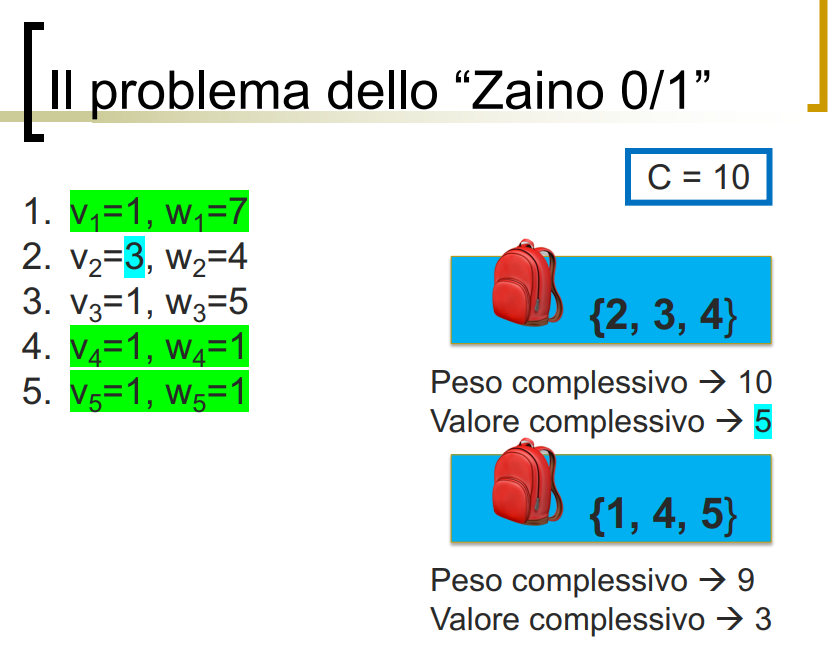
\includegraphics[width=100mm, scale=0.5]{chapters_ulerich/img/knapsack_example.png}
\end{center}
\section{Definizione formale}
Dato un insieme $X=\{1,2,\dots,i,\dots,n\}$ di n oggetti, un intero C e due funzioni:
\begin{itemize}
    \item $V:X \rt N$ tale che $V(i) = v_i$ è il valore dell'oggetto i
    \item $W:X \rt N$ tale che $W(i)=w_i$ è il peso dell'oggetto i
\end{itemize}
si vuole trovare un sottoinsieme $S=\{i_1,i_2,\dots, i_k\}$ di X tale per cui:
\begin{align*}
    W_S=&\sum^k_{j=1}w(i_j) \leq C\\
    V_S=&\sum^k_{j=1}v(i_j)
\end{align*}
Dove $V_S$ è il massimo tra tutti i valori dei possibili sottoinsiemi di X che sono "compatibili" con lo zaino.\\
Si tratta dunque di un problema di ottimizzazione di massimo, dove:
\begin{itemize}
    \item (n,C) \ra dimensione del problema
    \item Soluzioni possibili \ra tutti i sottoinsiemi $S'$ di X il cui peso totale $W_{S'}$ è al più la capacità C
    dello zaino
    \item Funzione obiettivo \ra valore totale $V_{S'}$ della soluzione possibile $S'$.
    \item Valore totale di S \ra valore ottimo
    \item S \ra Soluzione ottimale
\end{itemize}
\subsection{Soluzione del problema DP}
\begin{enumerate}
    \item Calcolo del valore ottimo (valore totale di S)
    \item Ricostruzione di una soluzione ottimale (un insieme S)
\end{enumerate}
\section{Sottostruttura Ottima}
Consideriamo l'esempio di inizio capitolo:
\begin{center}
    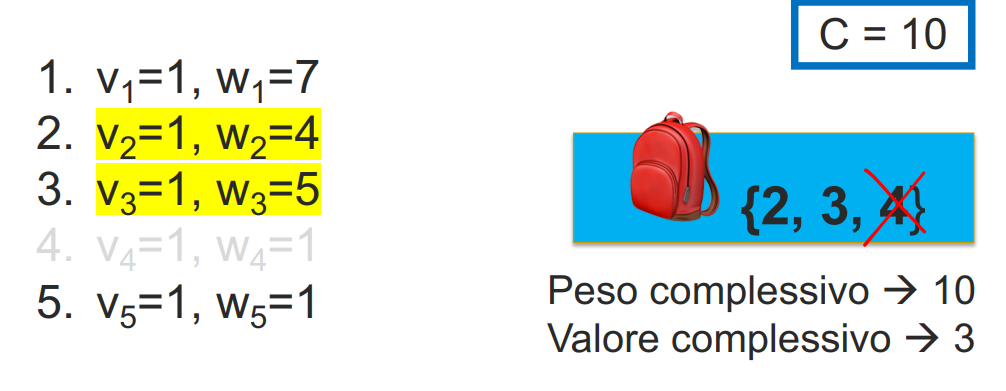
\includegraphics[width=80mm, scale=0.5]{chapters_ulerich/img/knapsack_ricerca_sott_ott.png}
\end{center}
$\{2,3\}$ è una soluzione ottimale di $X \setminus \{4\}$? \textcolor{red}{NO}.\\
$\{2,3, 5\}$ è una soluzione ottimale di $X \setminus \{4\}$!\\
\subsection{Diamo un ordine agli oggetti}
Diamo un ordine agli oggetti all'interno di X, cioè:\\
1 viene prime di 2 che viene prima di 3, etc. che viene prima dell'ultimo oggetto n.\\
\paragraph*{Data una soluzione ottima S si può verificare}
\begin{itemize}
    \item \textbf{CASO 1}: l'oggetto n appartiene a S
    \item \textbf{CASO 2}: l'oggetto n NON appartiene a S
\end{itemize}
\subsection*{CASO 1 $C \geq w_n$ e l'oggetto n appartiene a S}
\paragraph*{NB:} $S' = S \setminus \{n\}$ non è necessariamente la soluzione ottimale dell'istanza per
$X \setminus \{n\}$ e capacità C.\\
Infatti, se esiste $i \in X \setminus \{n\} \text{ t.c } i \notin S' \text{ e } w_i \leq C - W_{S'} 
\implies S' \cup \{i\}$ ha valore totale maggiore di quello di $S'$.\\
Tornando a noi, CASO 1 implica che $\implies S' = S \setminus \{n\}$ è soluzione ottimale per 
l'istanza data da:
\begin{itemize}
    \item insieme di oggetti $X \setminus \{n\} = \{1,2,\dots,n-1\}$
    \item Zaino di capacità $C'$ pari a $C-w_n$
\end{itemize} 
\begin{center}
    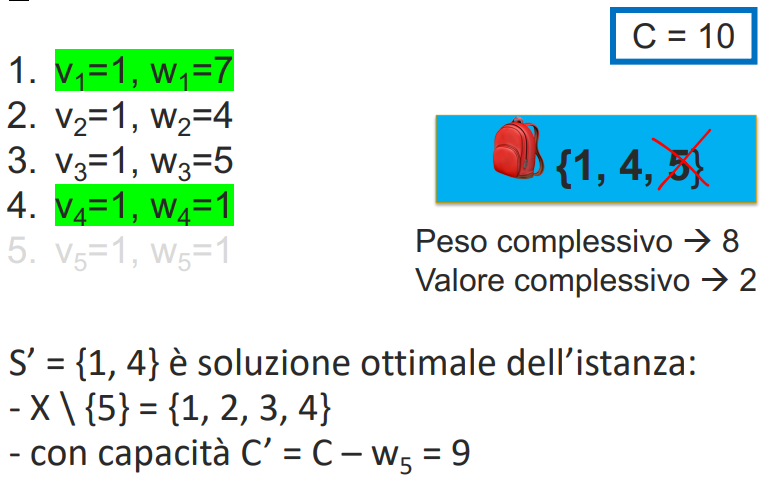
\includegraphics[width=90mm,scale=0.5]{chapters_ulerich/img/knapsack_n_in_S.png}
\end{center}
\subsection*{PROOF} 
\begin{enumerate}
    \item $S'$ è compatibile con la capacità $C-w_n$\\
    $W_S \leq C \implies W_S - w_n \leq C - w_n \implies W_{S'} \leq C- w_n$
    \item $S'$ ha valore totale $V_{S'}$ massimo\\
    Se esiste $S''$ tale che $V_{S''} > V_{S'}$ e $W_{S''} \leq C-w_n$\\
    $\implies S'' \cup \{n\}$ è soluzione ottimale per l'istanza X e C di valore totale
    maggiore di $V_S$ (contro l'ipotesi)
\end{enumerate}
\subsection*{CASO 2 - L'oggetto n NON appartiene a S}
$\implies$ S è soluzione ottimale per l'istanza data da:
\begin{itemize}
    \item insieme di oggetti $X \setminus \{n\} = \{1,2,\dots,n-1\}$
    \item Zaino di capacità pari a C
\end{itemize}
Non avendo aggiunto l'oggetto allo zaino la capacità totale rimane invariata.
\begin{center}
    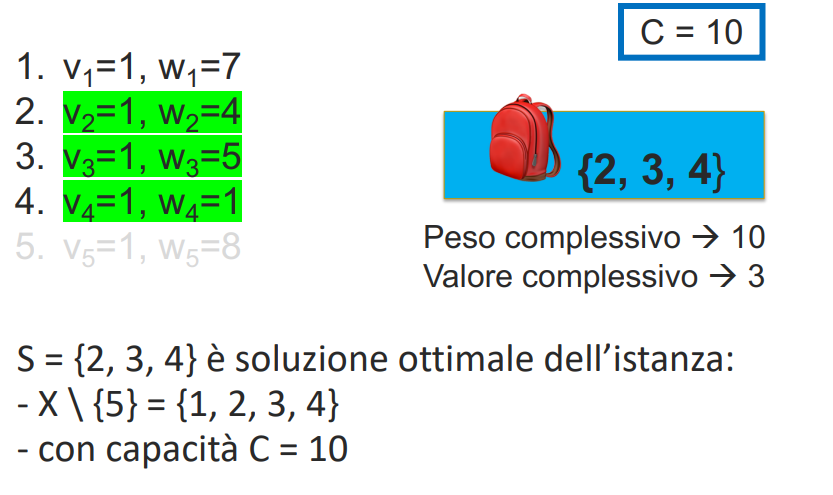
\includegraphics[width=90mm,scale=0.5]{chapters_ulerich/img/knapsack_n_notin_S.png}
\end{center}
\subsection*{PROOF}
Se esiste $S'$ che è soluzione ottimale per $X \setminus \{n\}$ e capacità C e con
valore $V_{S'} > V_{S'}$ allora $S'$ sarà soluzione ottimale per X e capacità C (contro
l'ipotesi).
\subsection{Sottostruttura ottima}
Dato un insieme $X=\{1,2,\dots,n\}$ di n oggetti, uno zaino di capacità C e una soluzione
ottimale S:\\
$C \geq w_n, \, n \in S \implies S' = S \setminus\{n\}$ è soluzione ottimale per:
\begin{itemize}
    \item insieme di oggetti $\{1,2,\dots, n-1\}$
    \item capacità $C-w_n$
\end{itemize}
\begin{mdframed}[backgroundcolor=lightgray]
    Problema $(n-1, C-w_n)$    
\end{mdframed}
\textbf{$S = S' \cup \{n\}$} con $S'$ soluzione ottimale per le condizioni viste prima del box.
$n \notin S \implies S$ è soluzione ottimale per:
\begin{itemize}
    \item insieme di oggetti $\{1,2,\dots,n-1\}$
    \item capacità C
\end{itemize}
\begin{mdframed}
    Problema $(n-1,C)$
\end{mdframed}
$S = S''$ con $S''$ soluzione ottimale per le condizioni viste prima del box.
\subsection{Passo ricorsivo per (n,C)}
Dato un insieme $X=\{1,2,\dots,n\}$ di n oggetti e uno zaino id capacità C, la soluzione
ottimale $S_{n,C}$ è:\\
\textbf{Se $C \geq w_n$ allora}
\begin{itemize}
    \item $S_{n,C} = max_V\{S' \cup \{n\},S''\}$
\end{itemize}
\textbf{altrimenti}
\begin{itemize}
    \item $S_{n,C} = S''$
\end{itemize}
$S'$ soluzione ottimale per il problema $(n-1, C-w_n) \rt S_{n-1,C-w_n}$\\
$S''$ soluzione ottimale per il problema $(n-1,C) \rt S_{n-1,C}$
Sostituisco nelle equazioni $S'$ e $S''$:
\textbf{Se $C \geq w_n$ allora}
\begin{itemize}
    \item $S_{n,C} = max_V\{S_{n-1, C-w_n} \cup \{n\},S_{n-1, C}\}$
\end{itemize}
\textbf{altrimenti}
\begin{itemize}
    \item $S_{n,C} = S_{n-1,C}$
\end{itemize}
\subsection{Definizione dei sottoproblemi}
\paragraph*{Sottoproblema di dimensione (i,c)}
Riempire uno zaino di capacità c con oggetti dall'insieme $\{1,2,\dots,i\} \rt S_{i,c}$\\
$i \in \{1,2,\dots,n\}$\\
$c \in \{0,1,\dots,C\}$
\paragraph*{Numero di sottoproblemi:}$(n+1)(C+1)$
\begin{mdframed}[backgroundcolor=yellow]
    $i=n,\, c=C$ \ra problema principale
\end{mdframed}
\section{Equazioni di ricorrenza}
\paragraph*{CASI BASE} \ra Tutti i sottoproblemi di dimensione $(i,c)$ tale per cui i = 0, oppure
C = 0.
\[S_{i,C} = \emptyset\]
\paragraph*{PASSO RICORSIVO} \ra Tutti i sottoproblemi di dimensione $(i,c)$ tale per cui
$i>0$ e $c>0$.\\
\textbf{Se $C \geq w_n$ allora}
\begin{itemize}
    \item $S_{n,C} = max_V\{S_{n-1, C-w_n} \cup \{n\},S_{n-1, C}\}$
\end{itemize}
\textbf{altrimenti}
\begin{itemize}
    \item $S_{n,C} = S_{n-1,C}$
\end{itemize}
Convertito in Equazioni di Ricorrenza:\\
\textbf{$i=0 \vee c=0$ (CASI BASE)}\\
$S_{i,c} = \emptyset$
\textbf{$i>0 \wedge c>0$ (PASSO RICORSIVO)}\\
$c \geq w_i \implies S_{i,c} = max_V\{S_{i-1,C-w_i} \cup \{i\},\,S_{i-1,C}\}$\\
$c < w_i \implies S_{i,c} = S_{i-1,C}$\\
\begin{mdframed}[backgroundcolor=yellow]
    $d_{i,c} \rt$ valore totale di $S_{i,c}$
\end{mdframed}
\subsection{Sostituzione coefficienti}
Sostituendo quindi $d_{i,c}$ a $S_{i,c}$ otteniamo:
\textbf{$i=0 \vee c=0$ (CASI BASE)}\\
$d_{i,c} = \emptyset$
\textbf{$i>0 \wedge c>0$ (PASSO RICORSIVO)}\\
$c \geq w_i \implies d_{i,c} = max_V\{d_{i-1,C-w_i} \cup \{i\},\,d_{i-1,C}\}$\\
$c < w_i \implies d_{i,c} = d_{i-1,C}$\\
\subsection{Calcolo dell'ottimo}
\begin{itemize}
    \item Si calcolano i coefficienti $d_{i,c}$ per dimensione $(i,c)$ crescente
    a partire dai casi base per $i=0$ e $c=0$
    \item Si memorizza $d_{i,c}$ ogni volta che si calcola l'ottimo per il sottoproblema $(i,c)$
    \item Quando si arriva a calcolare $d_{n,C}$ si ha il valore ottimo del problema $(n,C)$ 
\end{itemize}
\section{Algoritmo DP (bottom-up)}
\begin{enumerate}
    \item Costruzione di una matrice $D[0\dots n, 0\dots C]$
    \item Riempimento di D in modo tale che $D[i,c] = d_{i,c}$
    \item Valore ottimo \ra $D[n,C]$
\end{enumerate}
Avrò quindi la seguente matrice:
\begin{center}
    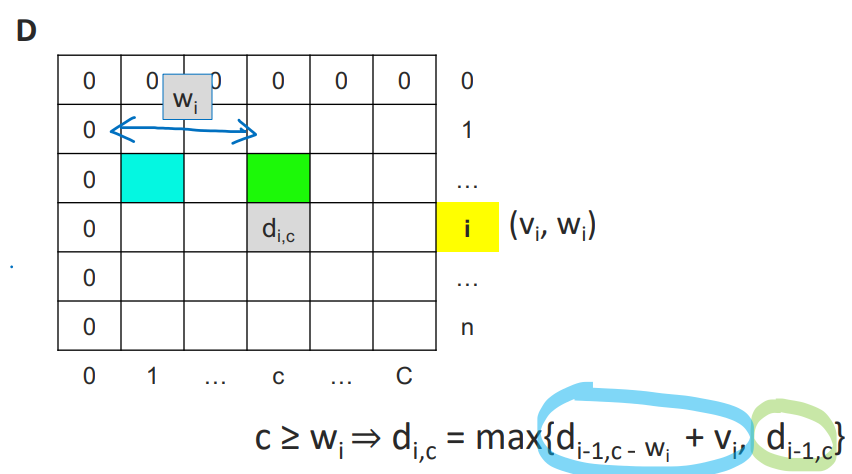
\includegraphics[width=80mm,scale=0.5]{chapters_ulerich/img/knapsack_matrix.png}
\end{center}
Dove sulle righe avrò il numero di oggetto con associato relativo valore $v_i$ e peso $w_i$.\\
Sulle colonne avrò capacità da 0 a C, che rappresenteranno i vari sottoproblemi, gli zaini più
piccoli.\\
Ricordiamo che abbiamo i seguenti oggetti:
\begin{enumerate}
    \item $v_1 = 1,\, w_1 = 7$
    \item $v_2 = 1,\, w_2 = 4$
    \item $v_3 = 1,\, w_3 = 5$
    \item $v_4 = 1,\, w_4 = 1$
    \item $v_5 = 1,\, w_5 = 1$
\end{enumerate}
Capacità $C=10$.
\subsection{Riempimento matrice}
Prima di tutto riempio la prima riga e colonna con 0 dato che rappresentano l'oggetto 0 e il
sottoproblema con $C=0$, sono i casi base.\\
Prendo il primo oggetto:
\begin{center}
    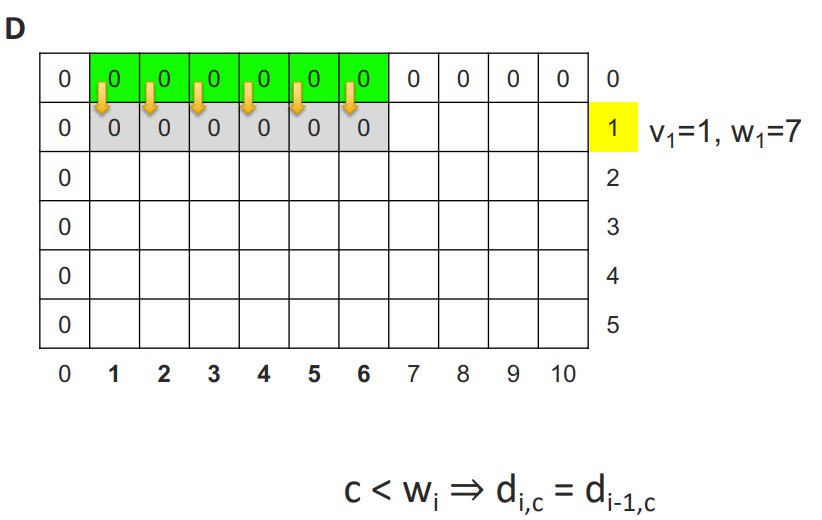
\includegraphics[width=80mm,scale=0.5]{chapters_ulerich/img/knapsack_matrix_filling_v1.png}
\end{center}
Notiamo che riempiamo di 0 la riga fino a quando non abbiamo $w_1 = c_i = 7$.\\
Qua controllo quale sia il massimo tra $d_{i-1,c-w_i} + v_i$ e $d_{i-1,c}$, cioè controllo se mi
conviene riempire lo zaino inserendo l'oggetto che sto considerando sommato con il valore dell'oggetto
precedente (considerando $c-w_i$, quindi un peso che non superi la capacità), oppure mi conviene riempire lo
zaino con la riga precedente perchè ha valore maggiore rispetto all'aggiunta del mio oggetto.\\
Proseguo così fino a riempire tutta la matrice, il valore ottimo sarà in fondo alla matrice a destra (come per LCS).
\begin{center}
    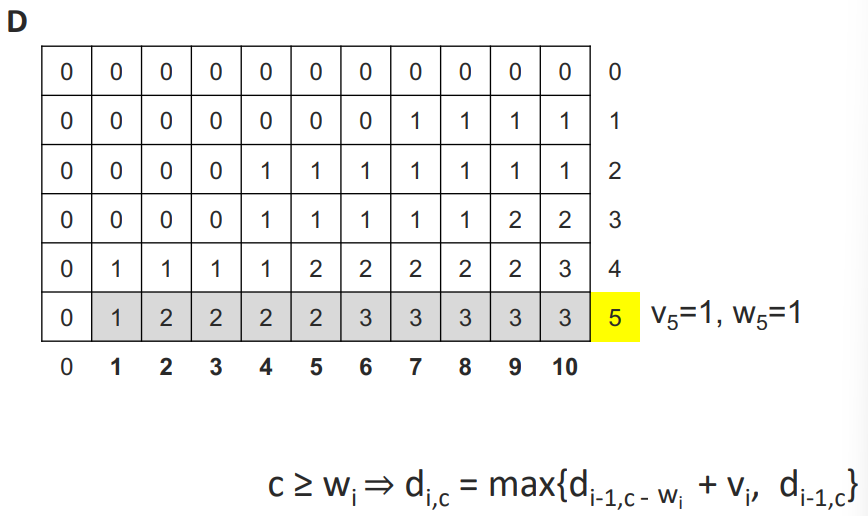
\includegraphics[width=80mm,scale=0.5]{chapters_ulerich/img/knapsack_matrix_filled.png}
\end{center}
%Arrivato a slide 154, ripassa riempimento matrice e poi scrivi codice


\chapter{Problema dei cammini minimi - Floyd-Warshall}
Come al solito diamo qualche definizione per poter lavorare successivamente in maniera
agile.
\section{Definizioni}
\subsection{Grafo}
Un Grafo viene definito come $G=(V,E)$ dove:
\begin{itemize}
    \item $V = \{v_1,v_2,v_3,...,v_n\}$ insieme di vertici
    \item $E= \{e_1,e_2,e_3,...,e_m\}$ insieme di archi
\end{itemize}
\paragraph*{Dimensione di G} $\rightarrow$ (n,m).
Arco $e_k \rightarrow$ relazione R tra due vertici $v_i$ e $v_j$
\paragraph*{R può essere}
\begin{itemize}
    \item Simmetrica - Grafo NON Orientato - cioè $v_i \, R \, v_j \Leftrightarrow v_j \, R \, v_i$
    \item Asimmetrica - Grafo Orientato (o diretto) - cioè $v_i \, R \, v_j \nLeftrightarrow  v_j \, R \, v_i$
\end{itemize}
Un grafo orientato è caratterizzato da un verso di percorrenza degli archi unidirezionale.
In questo caso E è sottoinsieme di $V^2$.
\begin{center}
    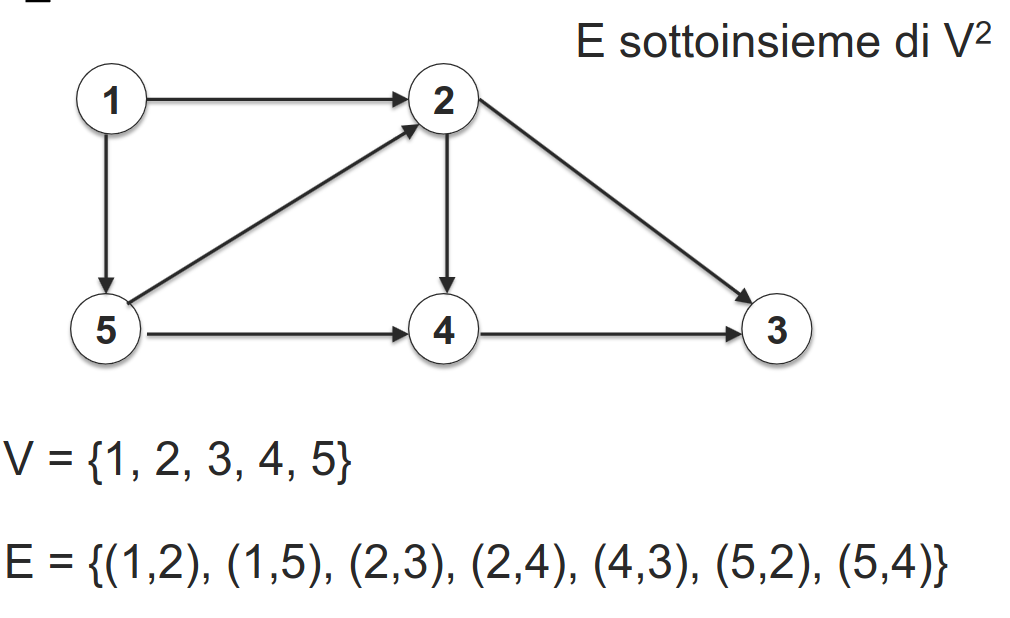
\includegraphics[width=80mm, scale=0.5]{grafo_orientato.png}
\end{center}
\begin{center}
    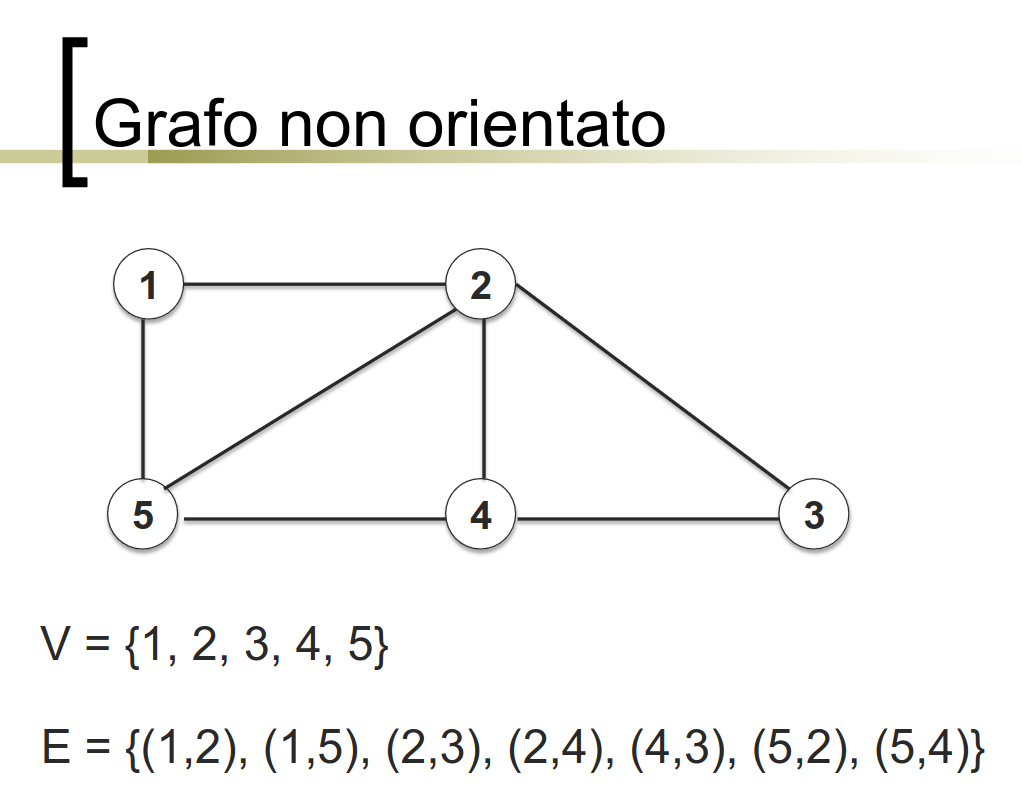
\includegraphics[width=80mm, scale=0.5]{grafo_non_orientato.png}
\end{center}
\subsection{Adiacenza}
Un vertifica v è adiacente a un vertice u se $(u,v)\in E$.\\
Per esempio nella rappresentazione del grafo orientato il vertice \textbf{1} è adiacante ai
vertici \textbf{2 e 5}, infatti notiamo che in E è presente $(1,2), (1,5)$.
\subsection{Rappresentazione di un grafo}
Abbiamo 2 rappresentazioni possibili:
\begin{itemize}
    \item Liste di adiacenza
    \item Matrice di adiacenza
\end{itemize}
\begin{enumerate}
    \item Le liste di adiacenza utilizzano un vettore $L_v$ di dimensione $|V|$ tale che $V[i]$ è la lista degli
    adiacenti del vertice $v_i$. Ogni vertice del grafo avrà un vettore.
    \item La matrice di adiacenza è una Matrice $M_v$ di dimensione $n \times n$ tale che $M[i,j] = 1$ se il
    vertice j è adiacente del vertice i, altrimenti $M[i,j] = 0$. A differenza delle liste in questo caso ho una sola
    matrice.
\end{enumerate}
\subsection{Esempio grafo orientato}
\begin{center}
    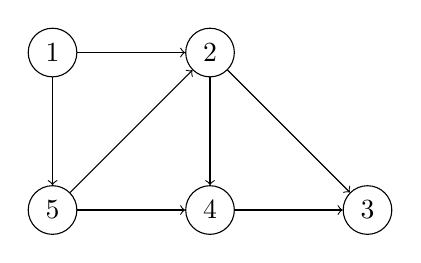
\begin{tikzpicture}
        \node[shape=circle,draw=black] (1) at (0,0) {1};
        \node[shape=circle,draw=black] (2) at (2,0) {2};
        \node[shape=circle,draw=black] (3) at (4,-2) {3};
        \node[shape=circle,draw=black] (4) at (2,-2) {4};
        \node[shape=circle,draw=black] (5) at (0,-2) {5};

        \path [->] (1) edge node[left] {} (2);
        \path [->] (2) edge node[left] {} (3);
        \path [->] (1) edge node[left] {} (5);
        \path [->] (5) edge node[left] {} (2);
        \path [->] (2) edge node[left] {} (4);
        \path [->] (5) edge node[left] {} (4);
        \path [->] (4) edge node[left] {} (3);

    \end{tikzpicture}
\end{center}

\begin{equation*}
    M = \begin{array}{c|ccccc}
    & 1 & 2 & 3 & 4 & 5 \\
    \hline
    1 & 1 & 0 & 0 & 1 & 0 \\
    2 & 0 & 0 & 1 & 1 & 0 \\
    3 & 0 & 0 & 0 & 0 & 0 \\
    4 & 0 & 1 & 0 & 0 & 0 \\
    5 & 1 & 0 & 1 & 0 & 0 \\
    \end{array}
\end{equation*}
\paragraph*{Dimensione} $|V|^2=n^2$
\paragraph*{Numero di celle con 1} $|E|$

\subsection{Esempio grafo non orientato}
\begin{center}
    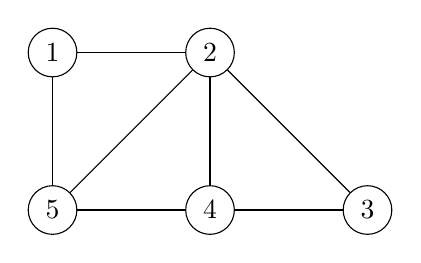
\begin{tikzpicture}
        \node[shape=circle,draw=black] (1) at (0,0) {1};
        \node[shape=circle,draw=black] (2) at (2,0) {2};
        \node[shape=circle,draw=black] (3) at (4,-2) {3};
        \node[shape=circle,draw=black] (4) at (2,-2) {4};
        \node[shape=circle,draw=black] (5) at (0,-2) {5};

        \path [-] (1) edge node[left] {} (2);
        \path [-] (2) edge node[left] {} (3);
        \path [-] (1) edge node[left] {} (5);
        \path [-] (5) edge node[left] {} (2);
        \path [-] (4) edge node[left] {} (2);
        \path [-] (5) edge node[left] {} (4);
        \path [-] (4) edge node[left] {} (3);

    \end{tikzpicture}
\end{center}

\begin{center}
    \begin{equation*}
        M = \begin{array}{c|ccccc}
          & 1 & 2 & 3 & 4 & 5 \\
        \hline
        1 & 0 & 1 & 0 & 0 & 1 \\
        2 & 1 & 0 & 1 & 1 & 1 \\
        3 & 0 & 1 & 0 & 1 & 0 \\
        4 & 0 & 1 & 1 & 0 & 1 \\
        5 & 1 & 1 & 0 & 1 & 0 \\
        \end{array}
        \end{equation*}
\end{center}
\paragraph*{Dimensione} $|V|^2=n^2$
\paragraph*{Numero di celle con 1} $2|E|$
\subsection{Liste VS Matrice (memoria)}
\paragraph*{Liste di adiacenza} Sono ottime dal punto di vista dell'occupazione dello spazio 
nel caso di Grafi sparsi con $|E|$ molto minore di $|V|^2$.
\paragraph*{Matrici di adiacenza} Risultano migliori nei grafi densi quindi quando ho
$|E|$ che si avvicina a $|V|^2$.
\subsection{Liste VS Matrice (tempo)}
\paragraph*{(u,v)} Intendiamo se i 2 vertici sono collegati.
Come tempo intendiamo il tempo per stabilire se (u,v) appartiene ad E e i tempi
sono i seguenti:
\begin{itemize}
    \item Liste di adiacenza $\rightarrow O(|E|) = O(m)$
    \item Matrice di adiacenza $\rightarrow O(1)$
\end{itemize}
\subsection{Cammino in un grafo orientato}
\paragraph*{Definizione di cammino} Sequenza $P=<v_{i_1},v_{i_2},..., v_{i_{k-1}},v_{i_k}>$
tale che $v_{i_k}$ appartiene a V per $1\leq j \leq k$ e $(v_{i_j},v_{i_{j+1}})$ appartiene
ad E per $1 \leq j < k$.
\paragraph*{Lunghezza del cammino} $k-1$ (numero di archi)
\paragraph*{Ciclo} Cammino in cui $v_{i_1}$ coincide con $v_{i_k}$
\paragraph*{Cammino semplice} Cammino in cui ogni vertice è presente una volta sola (cioè non
contiene cicli)
\paragraph*{Predecessore di $v_{i_k}$ in P} Vertice di $v_{i_{k-1}}$
\subsection{Grafo orientato pesato}
\paragraph*{Grafo} $G = (V,E,W)$
\begin{itemize}
    \item $V = \{v_1,v_2,v_3,...,v_n\}$ insieme di vertici
    \item $E= \{e_1,e_2,e_3,...,e_m\}$ insieme di archi
    \item $W:E \rightarrow R$ tale che $W(v_i,v_j) = w_{ij}$ è il peso dell'arco
    $(v_i,v_j)$
\end{itemize}
\paragraph*{Peso di un cammino} Si tratta della somma dei pesi di tutti gli
archi, formalmente: $P=<v_{i_1},v_{i_2},...,v_{i_k}> \rightarrow \sum^{k-1}_{j=1}w(v_{i_j},v_{i_{j+1}})$
\subsection{Esempio grafo orientato pesato}
\begin{center}
    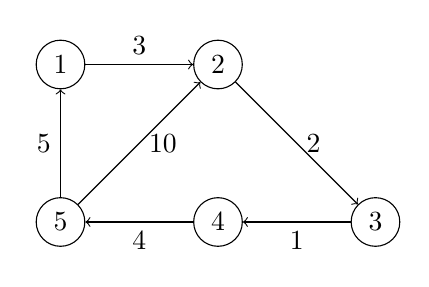
\begin{tikzpicture}
        \node[shape=circle,draw=black] (1) at (0,0) {1};
        \node[shape=circle,draw=black] (2) at (2,0) {2};
        \node[shape=circle,draw=black] (3) at (4,-2) {3};
        \node[shape=circle,draw=black] (4) at (2,-2) {4};
        \node[shape=circle,draw=black] (5) at (0,-2) {5};
    
        \path [->] (1) edge node[midway, above] {3} (2);
        \path [->] (2) edge node[midway, right] {2} (3);
        \path [->] (3) edge node[midway, below] {1} (4);
        \path [->] (4) edge node[midway, below] {4} (5);
        \path [->] (5) edge node[midway, left] {5} (1);
        \path [->] (5) edge node[midway, right] {10} (2);
        
    \end{tikzpicture}
\end{center}
\section{Il problema dei cammini minimi}
\paragraph*{Input} Grafo $G=(V,E,W)$ (senza cappi) orientato e pesato
\paragraph*{Output} Per ogni coppia di vertici i e j, trovare il cammino di peso minimo (cammino minimo)
che parte da i e finisce in j.\\
Si tratta di un problema di ottimizzazione di minimo, dove
\begin{itemize}
    \item (n) $\rightarrow$ dimensione del problema
    \item Soluzioni possibili per una coppia di vertici i e j sono tutti i cammini da i a j
    \item Funzione obiettivo è il peso del cammino
    \item Peso del cammino minimo da i a j è il valore ottimi (per i e j)
    \item Un cammino minimo tra i vertici i e j è la soluzione ottimale
\end{itemize}
\subsection{L'input}
\paragraph*{Funzione peso W} $W:E \rightarrow R^+$ tale che $W(i,j) = w_{ij} =$ peso dell'arco $(i,j)$.
\paragraph*{Funzione peso W - Versione estesa} $W:V \times V \rightarrow R^+$ tale che $W(i,j) = w_{ij}$ con:
\begin{itemize}
    \item $w_{ij} = 0$ se $i=j$
    \item $w_{ij} =$ peso dell'arco $(i,j)$, se $(i,j) \in E$
    \item $w_{ij} = \infty$, se $i \neq j$ e $(i,j) \notin E$ 
\end{itemize}
Matrice $W=[w_{ij}]$ di n righe e n colonne.
\subsection{L'output Matrici D e $\Pi$}
\begin{itemize}
    \item Matrice $D = [d_{ij}]$ di n righe e n colonne, dove $ [d_{ij}]$ è il peso del
    cammino minimo da i e j
    \item Matrice $\Pi = [\pi_{ij}]$ di n righe e n colonne, dove $\pi_{ij}$ è il predecessore di j
    nel cammino minimo da i a j
\end{itemize}
\paragraph*{Matrice D}
\begin{itemize}
    \item $d_{ij} = 0$ se $i = j$
    \item $d_{ij} = $ peso del cammino minimo, se esiste un cammino da i a j
    \item $d_{ij} = \infty$ se non esiste un cammino da i a j
\end{itemize}
\paragraph*{Matrice $\Pi$}
\begin{itemize}
    \item $\pi_{ij} = NIL$, se $i = j$
    \item $\pi_{ij} = u$ appartenente al cammino minimo da i a j, tale che $(u,j) \in E$, se
    esiste un cammino da i a j
    \item $\pi_{ij} = NIL$, se non esisto un cammino da i a j
\end{itemize}
Dopo aver riempito entrambe le matrici mi rendo conto che:\\
\textbf{La riga i d $\Pi$ fornisce l'albero dei predecessori relativo al vertice i}.
\paragraph{Albero dei predecessori del vertice i (riga i di $\Pi$)}
\begin{itemize}
    \item $\{ j \in V | \pi_{ij} \notin NIL\} \cup \{i\} \rightarrow$ insieme dei vertici
    \item ${(\pi_{ij}, j) | \pi{ij} \notin NIL}$
\end{itemize}
\section{Sosttostruttura ottima (primo tentativo)}
Consideriamo come $P_{ij}$ il \textbf{Cammino minimo da i a j} e p è il predecessore di j.\\
Sicuramente $P_{ij} = P_{ip} + <j>$, con $P_{ip}$ cammino minimo da i a p.
\begin{center}
    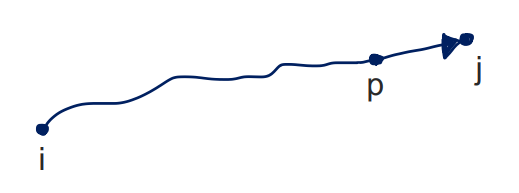
\includegraphics[width=70mm, scale=0.5]{chapters_ulerich/img/floyd_warshall_tent_sottostruttura.png}
\end{center}
Con $P_{ip}$ cammino minimo da i a p. Come potrei trovare $P_{ij}$?
\begin{center}
    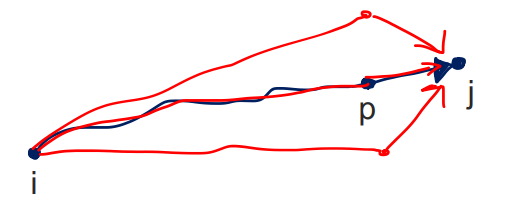
\includegraphics[width=70mm, scale=0.5]{chapters_ulerich/img/floyd_warshall_tent_sottostruttura_2.png}
\end{center}
\begin{enumerate}
    \item Considero tutti i vertici p' tali che $(p',j) \in E$
    \item Per ogni vertice p' determino il cammino dato da: $P_{ip} + <j>$
    \item Seleziono il cammino di peso minimo
\end{enumerate}
\paragraph*{Attenzione!} Non è sicuro che quando si calcola $P_{ij}$ si abbiano già a disposizione
i cammini $P_{ip'}$.
Si deve parametrizzare rispetto alla lunghezza I del cammino:
\begin{enumerate}
    \item Prima calcolo tutti i cammini minimi a lunghezza $0 \rightarrow P^0_{ij}$\\
    $P^0_{ij} = <i>$ se $i = j$, altrimenti $P^0_{ij} = \infty$
    \item Poi calcolo tutti i cammini minimi a lunghezza 1 $\rightarrow P^1_{ij}$\\
    $P^1_{ij} = <i,j>$ se $i \neq j$ e $(i,j) \in E$, altrimenti $P^1_{ij} = \infty$
    \item Poi calcolo tutti i cammini minimi a lunghezza 2 $\rightarrow P^2_{ij}$
    \item Poi calcolo tutti i cammini minimi a lunghezza 3 $\rightarrow P^3_{ij}$
    \item ...
    \item Ci si ferma per $l = |E| = m$ (l è lunghezza)
    \item Per ogni coppia i e j scelgo tra i cammini $P^0_{ij}, P^1_{ij}, \dots, P^m_{ij}$,
    quello di peso minimo
\end{enumerate}
\paragraph*{Friendly Reminder} $<i,j>$ Significa perorso con i vertici i e j.
\paragraph*{Domande} Come calcolo $P^l_{ij}$ con $l \geq 2$?\\
E qual è il tempo nel caso peggiore dell'algoritmo DP che sfrutta questa struttura ottima?\\
\subsection{Diamo un ordine ai vertici del grafo}
1 viene prima di 2 che viene prima di 3 etc. che viene prima dell'ultimo vertice n.\\
Parametriziamo rispetto ai vertici intermedi del cammino:
\begin{itemize}
    \item Trovo $P^0_{ij} \rightarrow$ cammino minimo senza vertici intermedi
    \item Trovo $P^1_{ij} \rightarrow$ cammino minimo con vertici intermedi $\in \{1\}$
    \item Trovo $P^2_{ij} \rightarrow$ cammino minimo con vertici intermedi $\in \{1,2\}$
    \item Trovo $P^3_{ij} \rightarrow$ cammino minimo con vertici intermedi $\in \{1,2,3\}$
    \item Trovo $P^n_{ij} \rightarrow$ cammino minimo con vertici intermedi $\in \{1,2,\dots,n\}$
\end{itemize}
\subsection*{Analizziamo nel dettaglio i cammini minimi intermedi}
$P^0_{ij} \rightarrow$ cammino minimo senza vertici intermedi.
\begin{align*}
  &P^0_{ij} = <i> \quad \text{se} \, i=j \\
  &P^0_{ij} = <i,j> \quad \text{se} \, i \neq j \text{ e } (i,j) \in E \\
  &P^0_{ij} = NIL \quad \text{se} \, i \neq j \text{ e } (i,j) \notin E
\end{align*}
Per $k > 0$, $P^k_{ij} \rightarrow$ cammino minimo con vertici intermedi $\in \{1,2,\dots,k\}$.\\
Per $k = n$, $P^n_{ij} \rightarrow$ cammino minimo con vertici intermedi $\in \{1,2,\dots,n\}$.\\
Quindi $P^n_{ij} \rightarrow$ cammino minimo $P_{ik}$.\\
\paragraph*{Sottoproblema di dimensione k} Per ogni coppia (i,j), trovare il cammino minimo
$P^k_{ij}$ dal vertice i al vertice j che ha vertici intermedi $\in \{1,2,\dots,k\}$ se $k>0$,
oppure non ha vertici intermedi se $k=0$.\\
\begin{align*}
    &k \in \{0,1,\dots,n\}\\
    &i \in \{1,\dots,n\}\\
    &j \in \{1,\dots,n\}
\end{align*}
\textbf{Numero di sottoproblemi} $n\times n \times (n+1)$.\\
$k = n \rightarrow P^n_{ij} = P_{ij}$.
\subsection{Equazioni di ricorrenza}
\paragraph*{Casi base} Sottoproblema di dimensione (0)
\begin{align*}
    &P^0_{ij} = <i> \quad \text{se } i = j\\
    &P^0_{ij} = <i, j> \quad \text{se } i \neq j \text{ e } (i,j) \in E\\
    &P^0_{ij} = NIL \quad \text{se } i \neq j \text{ e } (i,j) \notin E
\end{align*}
\paragraph*{Passo ricorsivo} Tutti i sottoproblemi di dimensione (k) tale che $k > 0$
\begin{align*}
    P^k_{ij} = ?
\end{align*}
Ricerchiamo la sottostruttura ottima.\\
\begin{center}
    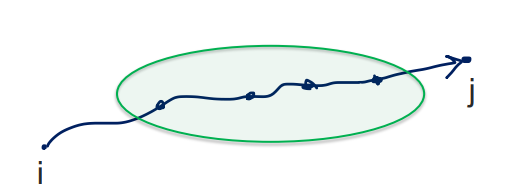
\includegraphics[width=70mm, scale=0.5]{chapters_ulerich/img/floyd_warshall_tent_sottostruttura_3.png}
\end{center}
\textbf{Data una soluzione ottimale $P_{ij}=P^n_{ij}$ si possono verificare due casi:}
\begin{enumerate}
    \item Il vertice n NON è uno dei vertici intermedi
    \item Il vertice n è uno dei vertici intermedi
\end{enumerate}
\subsection*{Caso 1 - Il vertice n NON è uno dei vertici intermedi}
\begin{itemize}
    \item $P^n_{ij}$ coincide con $P^{n-1}_{ij}$
    \item Predecessore di j in $P^n_{ij}$ coincide con predecesore di j in $P^{n-1}_{ij}$
\end{itemize}
\subsection*{Caso 2 - Il vertice n è uno dei vertici intermedi}
\begin{align*}
    P^n_{ij} = P_1 + P_2
\end{align*}
\begin{center}
    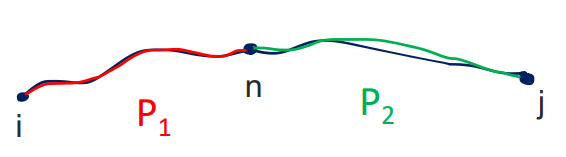
\includegraphics[width=70mm, scale=0.5]{chapters_ulerich/img/floyd_warshall_tent_sottostruttura_4.png}
\end{center}
\begin{align*}
    P_1 = P^{n-1}_{in} \rightarrow P^n_{ij} = P_1 + P_2 = P^{n-1}_{in} + P_2
\end{align*}
Mentre per quanto riguarda $P_2$ avrò che
\begin{align*}
    P_2 = P^{n-1}_{nj}
\end{align*}
Quindi sostituendo $P_2$ all'interno dell'equazione avrò che:
\begin{align*}
    P_2 = P^{n-1}_{nj} \rightarrow P^n_{ij} = P_1 + P_2 = P^{n-1}_{in} + P^{n-1}_{nj}
\end{align*}
Abbiamo quindi che il predecessore di j in $P^n_{ij}$ coincide con il predecessore di j in $P^{n-1}_{nj}$.\\
\subsection*{Passo ricorsivo per $P^n_{ij}$}
La soluzione ottimale $P^n_{ij} = P_{ij}$ è data da:
\[ P^n_{ij} = min_p\{P^{n-1}_{ij}, P^{n-1}_{in} + P^{n-1}_{nj}\} \]
$i = n$ oppure $j = n \rightarrow \, P^n_{ij} = P^{n-1}_{ij}$.
\subsection*{Passo ricorsivo per $P^k_{ij}$}
La soluzione ottimale $P^k_{ij} (k>0)$ è data da:
\begin{align*}
    P^k_{ij} = min_p{P^{k-1}_{ij}, P^{k-1}{ik} + P^{k-1}_{kj}}
\end{align*}
$i=k$ oppure $j=k \rightarrow \, P^k_{ij} = P^{k-1}_{ij}$.
\subsection{Equazioni di ricorrenza}
Riassumendo abbiamo le sequenti equazioni di ricorrenza:
\paragraph*{k=0 (CASI BASE)}
\begin{align*}
    &P^0_{ij} = <i> \quad \text{se } i = j\\
    &P^0_{ij} = <i, j> \quad \text{se } i \neq j \text{ e } (i,j) \in E\\
    &P^0_{ij} = NIL \quad \text{se } i \neq j \text{ e } (i,j) \notin E
\end{align*}
\paragraph*{$k>0$ (PASSO RICORSIVO)}
\begin{align*}
    P^k_{ij} = min_p{P^{k-1}_{ij}, P^{k-1}{ik} + P^{k-1}_{kj}}
\end{align*}
\subsection*{Definizione dei coefficienti}
\textbf{Coefficienti $d^k_{ij}$ dei sottoproblemi}.\\
$d^k_{ij} \rightarrow$ peso del cammino $P^k_{ij}$
\begin{align*}
    &k \in \{0,1,\dots,n\}\\
    &i \in \{1, \dots, n\}\\
    &j \in \{1,...,n\}
\end{align*}
Quindi abbiamo \textbf{Numero di coefficienti} uguale a $n \times n \times (n+1)$.\\
$k=n \rightarrow d^n_{ij}$ è il preso $d_{ij}$ di $P_{ij}$.\\
Ricordiamo che la funzione obiettivo è trovare il peso del cammino, definiamo quindi i
coefficienti nella seguente maniera:
\paragraph*{k=0 (CASI BASE)}
\begin{align*}
    &d^0_{ij} = 0 \quad \text{se } i = j\\
    &d^0_{ij} = w_{ij} \quad \text{se } i \neq j \text{ e } (i,j) \in E\\
    &d^0_{ij} = \infty \quad \text{se } i \neq j \text{ e } (i,j) \notin E
\end{align*}
\paragraph*{$k>0$ (PASSO RICORSIVO)}
\begin{align*}
    d^k_{ij} = min_p{d^{k-1}_{ij}, d^{k-1}{ik} + d^{k-1}_{kj}}
\end{align*}
\subsection*{Predecessori $\pi^k_{ij}$}
$\pi^k_{ij} \rightarrow$ predecessore del vertice j in $P^k_{ij}$
\begin{align*}
    &k \in \{0,1,\dots,n\}\\
    &i \in \{1, \dots, n\}\\
    &j \in \{1,...,n\}
\end{align*}
\textbf{Numero di predecessori}:: $n \times n \times (n+1)$.\\
$\pi^n_{ij} \rightarrow $ predecessore $\pi_{ij}$ di j in $P_{ij}$.\\
Aggiungiamo alle equazioni di ricorrenza anche i predecessori.
\paragraph*{k=0 (CASI BASE)}
\begin{align*}
    &d^0_{ij} = 0 \quad \pi^0_{ij} = NIL \quad \text{se } i = j\\
    &d^0_{ij} = w_{ij} \quad \pi^0_{ij} = i \quad \text{se } i \neq j \text{ e } (i,j) \in E\\
    &d^0_{ij} = \infty \quad \pi^0_{ij}= NIL \quad \text{se } i \neq j \text{ e } (i,j) \notin E
\end{align*}
\paragraph*{$k>0$ (PASSO RICORSIVO)}
\begin{align*}
    &d^k_{ij} = min_p{d^{k-1}_{ij}, d^{k-1}{ik} + d^{k-1}_{kj}}\\
    &\pi^k_{ij} = \pi^{k-1}_{ij} \text{ se } d^k_{ij} = d^{k-1}_{ij} \text{ altrimenti } 
    \pi^k_{ij} = \pi^{k-1}_{kj}
\end{align*}
\section{Algoritmo bottom-up}
Per ogni valore di k da 0 a n, vengono calcolate due matrici $(n\times n)$:
\begin{align*}
    &D^k=[d^k_{ij}]\\
    &\Pi^k=[\pi^k_{ij}]
\end{align*}
Il numero totale di matrici è $2(n+1)$.
\paragraph*{Caso Base} Ho che:
\begin{align*}
    &D^0=[d^0_{ij}] = W \text{ matrice dei pesi input}\\
    &\Pi^0=[\pi^0_{ij}]
\end{align*}
\paragraph*{Passo Ricorsivo} In questo caso ho:
\begin{align*}
    &D^k=[d^k_{ij}] \text{ e } \Pi^k=[\pi^k_{ij}]\\
    &\text{ Sono calcolate usando le matrici } D^{k-1} = [d^{k-1}_{ij}] \text{ e }
    \Pi^{k-1} = [\pi^{k-1}_{ij}]
\end{align*}
Avrò quindi che le matrici $D^n = [d^n_{ij}]$ e $\Pi^n = [\pi^n_{ij}]$ sono le matrici di
output!
\subsection{Algoritmo bottom-up - Codice}
\begin{lstlisting}[language=Java, escapeinside={*@}{@*}]
    Procedura calcola_valori_ottimi_FW(V,E,W)
      *@$D^0$@* = W
      *@$\Pi^0$@* = (n x n) matrix of NIL values
      for i = 1 to n do
        for j = 1 to n do
         if i != j and *@ $w_{ij}$ != $\infty$@* then
            *@ $\Pi^0$@* [i,j] = i
      for k = 1 to n do
        for i = 1 to n do
            for j = 1 to n do
                *@$D^k[i,j] = D^{k-1}[i,j]$@*
                *@$\Pi^k[i,j] = \Pi^{k-1}[i,j]$@*
                if i != k and j != k then
                    if *@$D^k[i,j]>D^{k-1}[i,k] + D^{k-1}[k,j]$@* then
                        *@$D^k[i,j] = D^{k-1}[i,k]+ D^{k-1}[k,j]$@*
                        *@$\Pi^k[i,j] = \Pi^{k-1}[k,j]$@*
\end{lstlisting}
\paragraph*{Tempo} $\Theta(n^3)$.
\subsubsection*{Rappresentazione esecuzione algoritmo}
Link al video \href{https://www.youtube.com/watch?v=4OQeCuLYj-4&ab_channel=MichaelSambol}{Youtube}.
\chapter{Algoritmi Greedy}
Si tratta di una tecnica che si applica sempre ai problemi di ottimizzazione, ma
rispetto alla programmazione dinamica ha un approccio diverso, dato che il calcolo della
soluzione ottima (in questo caso ne calcola una sola) avviene attraverso una
sequenza di scelte \textbf{localmente} ottime.
\paragraph*{Caratteristiche degli algoritmi Greedy}
\begin{itemize}
    \item Semplici da scrivere
    \item Efficienti
\end{itemize}
\paragraph*{Questioni}
\begin{itemize}
    \item Dimostrare la correttezza di un algoritmo greedy
    \item Capire quali problemi sono affrontabili con una strategia greedy
\end{itemize}
\section{Problema - Selezione attività}
\paragraph*{INPUT} Dato un insieme $A = \{a_1, a_2, \dots, a_n\}$ di n attività, tale
che $a_i = [s_i, e_i)$ per $\ \leq i \leq n$, dove $s_i$ è il tempo di inizio ed $e_i$ è il
tempo di fine.
\begin{center}
    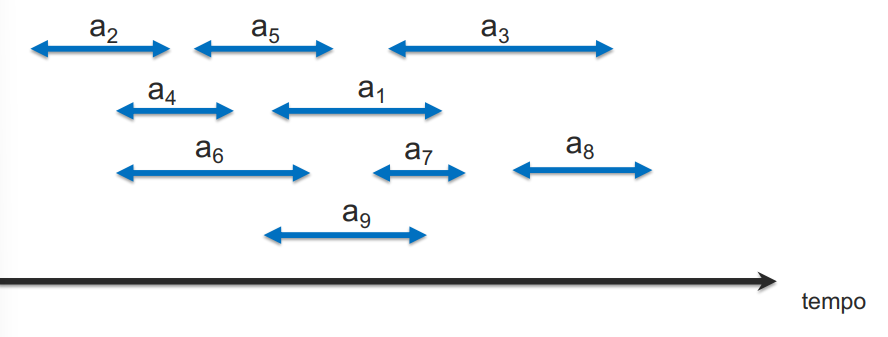
\includegraphics[width=80mm,scale=0.5]{greedy_sel_attivit.png}
\end{center}
$a_i=[s_i, e_i)$ e $a_j = [s_j, e_j)$ sono \textbf{compatibili} se $s_i \geq e_j$ oppure 
$s_j \geq e_i$. In poche parole se un attività inizia nello stesso momento della fine dell'altra, oppure dopo.
Le attività non devono accavallarsi, cioè eseguirsi nello stesso tempo di un'altra.
Facciamo qualche esempio che sicuramente è più semplice.\\
Per esempio $a_5=[s_5, e_5)$ e $a_8 = [s_8, e_8)$ sono compatibili, mentre $a_5 = [s_5, e_5)$ e 
$a_1 = [s_1, e_1)$ NON sono compatibili, infatti l'inizio di $a_1$ è minore della fine di $a_5$.
\paragraph*{OUTPUT} il sottoinsieme X di cardinalità massima composto di attività mutuamente compatibili.
In questo esempio l'OUTPUT desiderato è $X = \{a_2, a_5, a_7, a_8\}$.
\subsection{Soluzione con DP}
$A = \langle a_1, a_2,\dots,a_n\rangle$ tale che $e_1 \leq e_2 \leq \dots \leq e_n$.\\
$A = A \cup \{a_0, a_{n+1}\} = \langle a_0, a_1, \dots, a_n, a_{n+1}\rangle$ tale che $e_0 \leq s_1$
e $s_{n+1} \geq e_n$.
\paragraph*{Sottoproblema (i,j) per $0 \leq i < j \leq n+1$}
Trovare il sottoinsieme $X_{ij}$ di attività mutuamente compatibili di cardinalità massima per
$A_{ij} = \langle a_{i+1}, a_{i+2},\dots,a{j-2}, a{j-1} \rangle$.
\paragraph*{Sottoproblema $(0, n+1)$}
Trovare il sottoinsieme $X_{0,n+1} = X$ di attività mutuamente compatibili di cardinalità
massima per $A_{0,n+1} = \langle a_1, a_2, \dots, a_{n-1}, a_n \rangle = A$.\\
Numero totale di sottoproblemi \ra $(n+1)+n+(n-1)+(n-2)+\dots+1$.
\paragraph*{CASI BASE per $j=i+1 (A_{ij}=\emptyset)$}
$X_{ij} = \emptyset$.
\paragraph*{PASSO RICORSIVO per $j > i +1 (A_{ij} \neq \emptyset)$}
\textbf{Sottostruttura ottima}\\
$a_k$ appartiene a $X_{ij} \implies X_{ij} = X_{ik} \cup \{a_k\} \cup X_{kj}$\\
$X_{ik}$ soluzione ottima di $A_{ik}$\\
$X_{kj}$ soluzione ottima di $A_{kj}$\\
$X_{ij} = max\{X_ik \cup \{a_k\} \cup X_kj \text{ per } i < k < j\}$.
\paragraph*{Valore ottimo - Sostituzione coefficiente all'eqauzione}
\paragraph*{CASI BASE per $j=i+1 (A_{ij}=\emptyset)$}
$c_{ij} = 0$ (valore ottimo)
\paragraph*{PASSO RICORSIVO per $j > i +1 (A_{ij} \neq \emptyset)$}
$c_{ij} = max\{c_{ik} + 1 + c_kj \text{ t.c } i < k < j\}$ (valore ottimo).
\subsection{Svantaggi della Soluzione tramite DP}
\begin{enumerate}
    \item Tutti i sottoproblemi devono essere risolti per arrivare a calcolare il valore ottimo
    \item Si deve in seguito ricostruire la soluzione ottima (soluzione ottimale) perchè io ho solo
    i coefficienti, non ho la sequenza richiesta in OUTPUT
\end{enumerate}
\subsection{Approccio greedy}
\begin{center}
    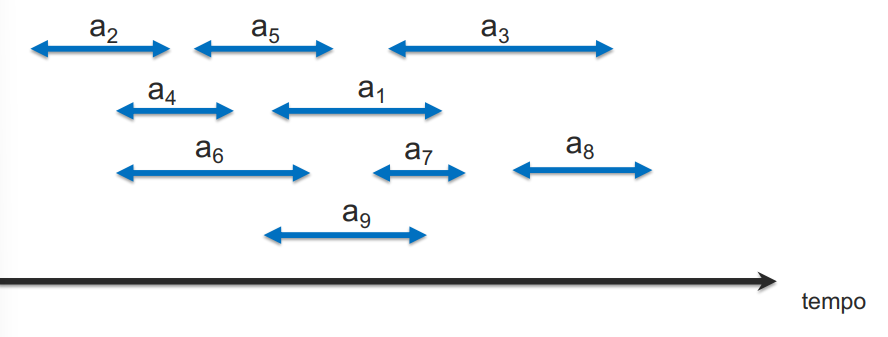
\includegraphics[width=80mm,scale=0.5]{greedy_sel_attivit.png}
\end{center}
In questo caso dobbiamo scegliere un parametro, per esempio \ra Attività con il tempo
di fine più basso, che in questo caso è $a_2$.\\
\textbf{IPOTESI}: $a_2$ appartiene alla soluzione ottima X $\implies X = \{a_2\} \cup X_2$.\\
\textbf{$X_2$ è la soluzione ottima per $A_2 = \{a = [s,e) \in A | \text{ a compatibile con } a_2\}$}
Compatibile con $a_2$ significa che $s \geq e_2$. Graficamente devo avere che la fine di $a_2$ non si
intersechi nessuna attività. Quindi devo cercare l'attività con il tempo di fine più basso in $A_2 \rt a_5$.
\begin{center}
    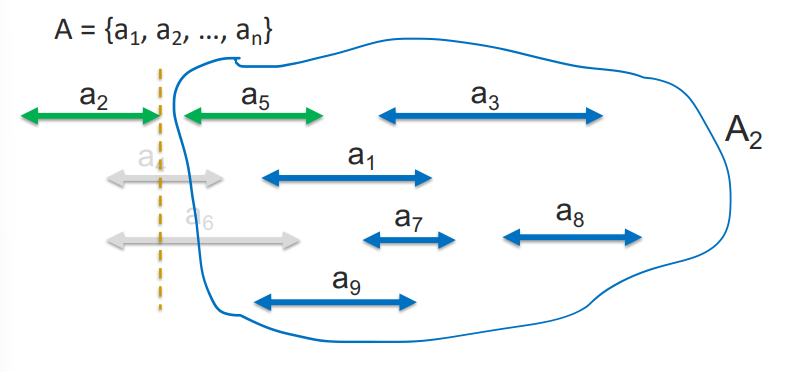
\includegraphics[width=80mm,scale=0.5]{greedy_sel_attivit_p2.png}
\end{center}
Scelgo quindi $a_5$ dato che ha il tempo di fine più basso rispetto a tutte le attività 
compatibili con $a_2$.\\
\textbf{IPOTESI} $a_5$ appartiene alla soluzione ottima $X_2 \implies X = \{a_2\} \cup \{a_5\} \cup X_2$.\\
$X_5$ è soluzione ottima per $A_5 = \{a=[s,e) \in A | s \geq e_5\}$.\\
Ancora una volta cerco le attività compatibili con $a_5$, che abbiano quindi un inizio che sia maggiore
o uguale rispetto alla fine di $a_5$, e scelgo quella con tempo di fine minore.\\
Determino quind che $A_5 \rt a_7$.\\
\textbf{IPOTESI}: $a_7$ appartiene alla soluzione ottima $X_5 \implies X = \{a_2\} \cup \{a_5\} \cup \{a_7\} \cup X_7$.\\
Cerco nuovamente l'attività con tempo di fine più basso rispetto a quelle compatibili con $a_7$ e trovo
che l'attività in questione è $a_8$.\\
\textbf{IPOTESI}: $a_8$ appartiene alla soluzione ottima $X_7$.\\
Quindi questo implica che $X = \{a_2\} \cup \{a_5\} \cup \{a_7\} \cup \{a_8\} \cup X_8$.\\
$X_8$ è soluzione ottima per $A_8 = \{a=[s,e) \in A\,t.c\, s \geq e_8\}$.\\
Ma dato che non ho più eventi compatibili con $a_8$ (perchè sono finiti, ma valeva anche il caso che c'erano altri
eventi che NON compatibili), $A_8 = \emptyset$. Significa che sono arrivato ad avere la soluzione
e guardandola notiamo che è una soluzione ottimale.\\
\[ X = \{a_2, a_5, a_7, a_8\} \]
\subsection{Osservazioni sulla risoluzione Greedy}
Notiamo che ad ogni passo la scelta localmente ottima minimizza il tempo di fine. Sono state effettuate
4 scelte localmente ottime, sono quindi stati risolti 4 sottoproblemi.\\
\paragraph*{In sintesi} Ad ogni passo:
\begin{enumerate}
    \item effettuo una scelta localmente ottima
    \item risolvo il sottoproblema generato dalla scelta appena effettuata
    \item la scelta non dipende dalle scelte successive (Greedy è anche detto algoritmo miope)
    \item la scelta riduceo il sottoproblema da risolvere (approccio Top-Down)
\end{enumerate}
\subsection{Codice Greedy}
\begin{lstlisting}[language=Java, escapeinside={@*}{*@}]
    Procedura greedy_scheduling(A)
        n = |A|
        @*$a_s$*@ = attivita' di A con il minore tempo di fine
        X = {@*$a_s$*@}
        @*$a_s$*@ = a=[s,t) t.c @*$s \geq e_s$*@ e minore tempo di fine
        while @*$a_s \neq NIL$*@ do
            X = @*$\{a_s\} \cup X$*@
            @*$a_s$*@ = a=[s,t] t.c @*$s \geq e_s$*@ e minore tempo di fine
        return X
\end{lstlisting}
Tempo di esecuzione $O(n)^2$, determinato dal While, perchè le altre
operazioni o sono costanti o nel caso della ricerca dell'evento compatibile
con tempo di fine minore impiegano tempo $O(n)$.
\paragraph*{Miglioramento} Posso migliorare l'algoritmo ordinando le attività di A per tempo di fine
non decrescente, prima di eseguire le operazioni di ricerca evento minimo, inserisco quindi un
tempo di $O(n\log n)$ determinato dall'algoritmo di ordinamento (es. MergeSort o QuickSort).\\
\begin{enumerate}
    \item Ordine le attività di A per tempo di fine non decrescente
    \item Aggiungo $a_1$ alla soluzione ottima X
    \item Aggiungo a X la prima attività dopo $a_1$ che ha tempo di inizio $\geq e_1$
    \item Aggiungo a X la prima attività dopo la precedente che ha tempo di inizio $\geq$ al suo
    tempo di fine
    \item Aggiungo a X la prima attività dopo la precdente che ha tempo di inizio $\geq$ al suo tempo
    di fine
    \item Etc.
    \item Mi fermo quando ho considerato tutte le attività
\end{enumerate}
\begin{center}
    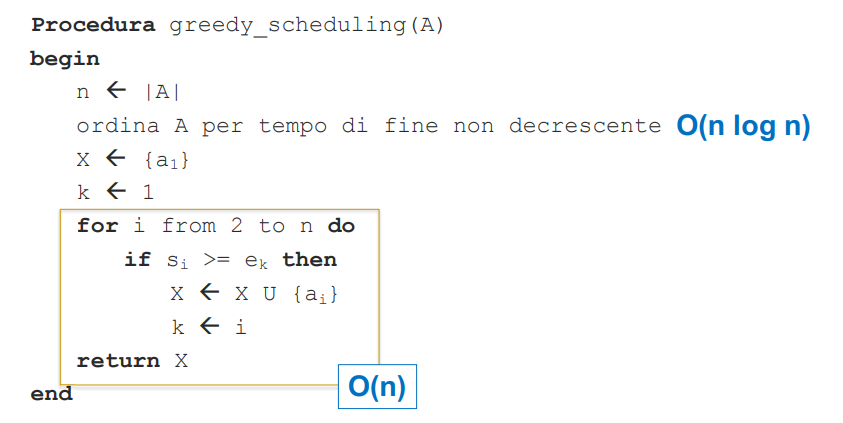
\includegraphics[width=80mm,scale=0.5]{greedy_code_ordinamento.png}
\end{center}
\section{Greedy VS DP}
\begin{itemize}
    \item Soluzione ottima \textbf{VS} Valore ottimo + Soluzione ottima
    \item Top-down \textbf{VS} Bottom-up
    \item Pochi sottoproblemi da risolvere \textbf{VS} Tanti sottoproblemi da risolvere
    \item Efficiente e semplice da scrivere \textbf{VS} Meno efficiente e più complicato da scrivere
    \item Applicabilità inferiore (te pareva) \textbf{VS} Applicabilità maggiore
\end{itemize}
\subsection{Due ingredienti chiave di un algoritmo Greedy}
\begin{itemize}
    \item Proprietà della sottostruttura ottima (tipica anche della Programmazione Dinamica)
    \item Proprietà della \textbf{scelta greedy}
\end{itemize}
Per la \textbf{Correttezza di un algoritmo Greedy} si deve DIMOSTRARE che la sequenza di scelte
localmente ottima conduce a una soluzione globalmente ottima.\\
\paragraph*{Proprietà della scelta greedy:} la scelta che compio ad ogni passo appartiene a una soluzione
ottima del sottoproblema che sto risolvendo in quel momento.
\section{Correttezza di un algoritmo Greedy}
Analizziamo la sottostruttura del problema della selezione di attività.
\paragraph*{Sottoproblema al passo generico:} Trovare il sottoinsieme di cardinalità massima di
attività compatibili, per l'insieme di attività che iniziano dopo la fine dell'attività aggiunta al passo
precedente.\\
\textbf{Sottoproblema 1}: sottoinsieme di cardinalità massima di attività compatibili,
per l'insieme A\\
\textbf{Sottoproblema 2}: sottoinsieme di cardinalità massima di attività compatibili, per 
l'insieme $A_2$ delle attività che hanno tempo di inizio $\geq$ al tempo di fine della
scelta fatta al passo 1.\\
...\\
\textbf{Sottoproblema k}: sottoinsieme di cardinalità massima di attività compatibili,
per l'insieme $A_k$ delle attività che hanno tempo di inizio $\geq$ al tempo di fine della
scelta fatta al passo $k-1$.\\
Scelta localmente ottima per il sottoproblema k \ra Attività $a_s$ con il minor tempo di fine
$A_k$.
\paragraph*{Proprietà della scelta greedy da dimostrare}
Ad ogni passo l'attività scelta è inclusa in una soluzione ottima del sottoproblema che sto risolvendo.
Basta dimostrare che \textbf{$a_1$ è inclusa in una soluzione ottima per l'insieme A}.\\
\subsection*{Dimostrazione}
Suppongo X soluzione ottima per A. Suppongo $a'_1$ attività con il minore tempo di fine X.\\
Se $a'_1$ uguale ad $a_1$ la dimostrazione è finita, altrimenti sostituisco in X l'attività
$a'_1$ con $a_1$.\\
Le attività in X sono ancora disgiunte. La dimensione di X non è cambiata.\\
\textbf{Conclusione:} il nuovo X è un sottoinsieme massimo di attività compatibili di A che include
ora $a_1$. 
\subsection{Cosa succede se sbaglio parametro?}
Consideriamo per esempio la durata massima come parametro, cosa succede alle soluzioni?\\
Prendendo l'esempio precedente notiamo subito che gli eventi della soluzione sarebbero i più
lunghi quindi $a_3$ e $a_6$ e questa non è una soluzione ottima.\\
Se scegliamo la durata minima otteniamo che in ordine di scelta $a_7,\, a_4,\, a_8$,
anche in questo caso questa non è una soluzione ottima.\\
Ci accorgiamo inoltre che i valori scelti inizialmente non sono soluzione ottima del sottoproblema,
mi rendo conto abbastanza velocemente quindi che sto sbagliando, ma analizziamo nel dettaglio
la questione considerando il seguente problema. 
\section{Il problema dello Zaino Frazionario}
Dati n oggetti $\langle 1,2,\dots,n \rangle$, un intero C e due funzoni.
\begin{itemize}
    \item $V:X \rt N$   $V(i) = v_i$, valore dell'oggetto i
    \item $W:X \rt N$   $W(i) = w_i$, peso dell'oggetto i
\end{itemize}
Trovare una sequenza $P = \langle p_1, p_2, \dots, p_n \rangle$ con $p_i$ in $[0,1]$ per
$1 \leq i \leq n$, tale per cui:
\[ \sum^n_{i=1}p_i w_i \leq C \]
\[ \sum^n_{i=1}p_i v_i \rt \text{ massimo valore} \]
In questo caso, a differenza del problema dello zaino 0/1, posso scegliere di frazionare gli oggetti,
quindi non devo per forza prendere tutto l'oggetto, ma posso prenderne anche solo una parte.
\section{Possibile strategia Greedy}
\begin{itemize}
    \item Ordino gli oggetti per valore non crescente
    \item Prendo la maggiore quantità del primo oggetto compatibile con la capacità dello zaino
    \item Prendo la maggiore quantità del secondo oggetto compatibile con la capacità residua dello zaino
    \item Prendo la maggiore quantità del terzo oggetto compatibile con la capacità residua dello zaino
    \item etc.
    \item Mi fermo non appena lo zaino è completamente pieno
\end{itemize}
Vediamo se questa strategia funziona:
\paragraph*{Istanza Problema}
Oggetti \ra $\langle 1,2,3 \rangle$
\begin{enumerate}
    \item $v_1 = 10$, $w_1 = 20$
    \item $v_2 = 9$, $w_2 = 8$
    \item $v_3 = 8$, $w_3 = 5$
\end{enumerate}
La capacità totale $C = 20$, mentre $c$ è la capacità residua.\\
Proviamo inserendo quindi la maggiore quantità di oggetto con valore maggiore.\\
Inserisco quindi l'oggetto 1, avendo capacità 20 e peso 20 posso inserirlo tutto.\\
Avendo peso 20 ho saturato completamente la capacità dello zaino e ho un valore di 10,
ottengo quindi che la soluzione $P = \langle 1,0,0 \rangle$ con appunto Valore \ra 10.\\
\'E facile osservare che NON si tratta della soluzione ottima, questo significa che ho sbagliato
a scegliere il parametro per la strategia Greedy.
\subsection{Cambio parametro}
Se scegliessi iniziassi a riempire lo zaino considerando il rapporto tra peso e valore, otterrei
i seguenti valori:
\begin{enumerate}
    \item $v_1 = 10$, $w_1 = 20, \frac{v_1}{w_1} = 0.5$
    \item $v_2 = 9$, $w_2 = 8, \frac{v_2}{w_2} = 1.125$
    \item $v_3 = 8$, $w_3 = 5, \frac{v_3}{w_3} = 1.6$
\end{enumerate}
Risulta quindi evidente che conviene inserire prima l'oggetto 3 perchè posso inserire
più parti di oggetto e avere più valori rispetto a inserire lo stesso peso degli altri.\\
Inserisco quindi tutto il terzo oggetto, occupando capacità 5, inserisco quindi il secondo oggetto,
che ha rapporto peso valore maggiore rispetto al primo. Dopo aver inserito il secondo oggetto,
noto di avere ancora dello spazio disponibile, quindi procedo a inserire il primo oggetto che però
non è possibile inserire tutto, ne inserisco quindi peso 7, cioè la capacità residua.\\
Ottengo quindi $P = \langle 0.35, 1, 1 \rangle$ e Valore \ra 20.5 che oltre a essere un valore
maggiore del primo tentativo è soluzione ottima. Questo è quindi il parametro corretto.
\subsection{Strategia Greedy Attuata}
\begin{itemize}
    \item Calcolo per ogni oggetto i il valore specifico $v_i/w_i$
    \item Ordino gli oggetti per valore specifico non crescente
    \item Prendo la maggiore quantità del primo oggetto compatibile con la capacità
    dello zaino
    \item Prendo la maggiore quantità del secondo oggetto compatibile con la capacità
    residua dello zaino
    \item ...
    \item Mi fermo appena lo zaino è completamente pieno
\end{itemize}
\paragraph*{Generico passo i} Scelta localmente ottima \ra percentuale di oggetto
i-esimo da prendere $p_i = min(c/w_i,1)$.\\
c è C diminuita del peso totale degli oggetti da 1 a i-1.\\
Sottoproblema lasciato dalla scelta di $p_i$:
\begin{itemize}
    \item Oggetti da i+1 a n
    \item Capacità C diminuita del peso totale degli oggetti da 1 a i
\end{itemize}
\subsection{Codice}
Inserire Codice
% Manca Codice
\subsection{Proprietà della scelta Greedy (da dimostrare)}
La percentuale $p_i$ scelta per l'oggetto i è inclusa in una soluzione ottima relativa al
sottoproblema:
\begin{itemize}
    \item oggetti da i a n
    \item Capacità residua dello zaino pari a C diminuita del peso totale degli
    oggetti aggiunti da 1 a i-1
\end{itemize}
Basta dimostrare la proprietà per la percentuale $p_1$ e sottoproblema:
\begin{itemize}
    \item Oggetti da 1 a n
    \item Capacità C dello zaino
\end{itemize}
\section{Algoritmi Greedy in Generale}
\subsection{Codice generico}
\begin{lstlisting}[language=Java, escapeinside={@*}{*@}]
    Procedura general_greedy(S = {@*$s_1,s_2,...,s_n$*@})
        Calcola per ogni elemento un certo parametro
        Ordina S sulla base del parametro calcolato
        X = @*$\emptyset$*@
        for i from 1 to n do
            if @*$s_i$*@ is la scelta localmente ottima then
                X = @*$\{s_i\} \cup X$*@
        return X
\end{lstlisting}
\section{Non tutti i problemi ammettono un algoritmi Greedy}
Il problema zaino 0/1 non ammette un algoritmo di tipo greedy come soluzione.
Nelle slide vengono fatti degli esempi che mostrano che è impoddibile identificare
una strategia greedy valida.\\
Questo perchè non tutti i problemi ammettono un algoritmo Greedy, ma la vera questione
è: \textbf{Come capire, in linea di principio, se un problema ammette un algoritmo Greedy?}.\\
Per capire questo aspetto dobbiamo introdurre una struttura denominata Matroide.
\paragraph*{Matroide:} struttura combinatoria a cui è associato un algoritmo greedy.
\subsection{Sistema di Indipendenza}
Una coppia (S,F)
\begin{itemize}
    \item S, insieme finito $\{s_1, s_2, \dots, s_n\}$ di elementi
    \item F, una famiglia di sottoinsiemi di S, cioè un sottoinsieme dell'insieme P(S)
    delle parti di S
\end{itemize}
\paragraph*{Esempio} 
\begin{align*}
    &S = \{1,2,3\}\\
    &P(S) = \{\emptyset, \{1\},\{2\},\{3\},\{1,2\},\{1,3\},\{2,3\},\{1,2,3\}\}\\
    &F=\{\{1\},\{3\},\{1,3\}\}\\
\end{align*}
Una coppia (S,F) così definita è un \textbf{Sistema di Indipendenza} se vale la seguente
proprietà:\\
\textbf{preso $A \in F$ allora un qualsiasi $B \subseteq A$ appartiene a F}.\\
Elementi di F \ra sottoinsiemi indipendenti.\\
\paragraph*{Esempio}
\begin{itemize}
    \item S, insieme $\{1,2,...,n\}$ di n oggetti a cui è associato un peso
    \item F, famiglia dei sottoinsiemi di S che hanno peso totale $\leq$ C
\end{itemize}
è un Sistema di Indipendenza, cioè:\\
$A \in F, \, B \subseteq A \implies B \in F$\\
\paragraph*{PROOF:} Se $A \in F$, allora il suo peso totale è $\leq$ C.\\
Un qualsiasi $B \subseteq A$, avrà peso totale $\leq$ C e quindi anche $B \in F$.\\
\subsection{Proprietà di scambio}
Un sistema di Indipendenza (S,F) è un \textbf{matroide} se vale la seguente
\textbf{proprietà di scambio}:\\
\textbf{Per qualsiasi A, $B \in F$ tali che $|B|=|A|+1$, allora esiste almeno un elemento
$b \in B-A$ tale che $\{b\}\cup A \in F $}.\\
\paragraph*{NB} in un matroide l'insieme vuoto è un insieme indipendente.
\subsection{Esempio 1}
Coppia (S,F):
\begin{itemize}
    \item S, insieme finito di oggetti
    \item F, famiglia dei sottoinsiemi di S di cardinalità $\leq k$
\end{itemize}
(S,F) è un Sistema di Indipendenza, cioè:\\
$A \in F, \, B \subseteq A \implies B \in F$\\
\textbf{PROOF}: Se $A \in F$, allora la sua cardinalità è $\leq k$.\\
Un qualsiasi $B \subseteq A$ avrà cardinalità $\leq k$ e quindi anche $B \in F$.\\
\paragraph*{Proprietà Scambio} Per (S,F) vale la proprietà dello scambio, cioè:\\
\[ \forall A,b \in F \text{ t.c. } |B| = |A|+1 \implies \exists b \in B-A \text{ t.c } \{b\} \cup A \in F\]
\paragraph*{PROOF}
Se A e B $\in F$, allora $|A| \leq k$ e $|B| \leq k$, A ha un elemento in meno rispetto a B
quindi $|A| < k$.\\
Un qualsiasi $b \in B-A$ che viene aggiunto ad A produce un insieme di cardinalità $\leq k$,
che quindi appartiene a F.
\subsection{Esempio 2}
\textbf{Coppia S,F}:
\begin{itemize}
    \item S, insieme E degli archi di un grafo non orientato
    \item F, famiglia dei sottoinsiemi di S composti da archi che hanno un vertice in comune
\end{itemize}
(S,F) è un Sistema di Indipendenza, cioè:\\
\[A \in F, B \subseteq A \implies B \in F\]
\paragraph*{PROOF} Se $A \in F$, allora A è composto da archi incidenti in un vertice v.\\
Un qualsiasi $B \subseteq A$ sarà composto di archi incidenti in v e quindi anche $B \in F$.
\paragraph*{Proprietà dello scambio} Per (S,F) NON vale la proprietà dello scambio cioè:
\[ \forall A,B \in F \text{ t.c. } |B|=|A|+1 \nrightarrow \exists b \in B-A \text{ t.c. } \{b\} \cup A \in F\]
\paragraph*{PROOF} A e B potrebbero riferirsi a due vertici diversi.\\
CONTROESEMPIO: $A = \{(5,6) e (6,7)\}$ e $B = \{(2,3)(3,4),(3,5)\}$.
\paragraph*{Esempio 3} Nelle slide c'è un terzo esempio riguardo l'insieme finito di vettori
di uno spazio vettoriale (S) e la famiglia dei sottoinsiemi di S composti da vettori 
linearmente indipendenti (F).
\section{Matroide Grafico $M_G$}
Dato un grafo $G=(V,E)$ non orientato e connesso $M_G = (S,F)$ con:
\begin{itemize}
    \item S, insieme E degli archi
    \item F, tutti i sottoinsiemi di S che sono aciclici
\end{itemize}
è il \textbf{matroide grafico} relativo a G.\\
$A \in F \implies G_A = (V,A)$ è una \textbf{foresta}.
%Arrivato a slide 46
\chapter{Minimum Spanning Tree - MST}
\paragraph*{INPUT}: Grafo connesso non orientato pesato $G=(V,E)$ con:\\
$W:E \rt R^+$ tale che $W(u,v)$ è il peso dell'arco (u,v).
\paragraph*{OUTPUT}: $T \subseteq E$ aciclico tale che:
\begin{enumerate}
    \item $\forall v \in V, \exists (u,v) \in T$
    \item $W(T) = \sum_{(u,v)\in T} W(u,v)$ è minimo
\end{enumerate}
$G_T = (V,T) \rt$ Minimum Spanning Tree (MST).
\begin{center}
    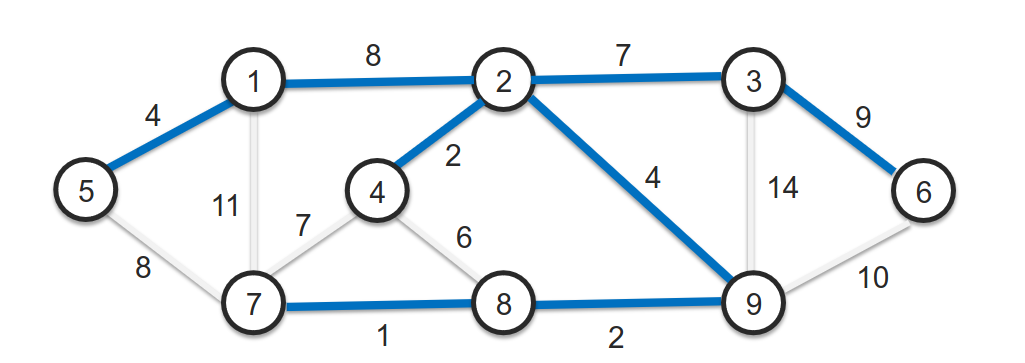
\includegraphics[width=80mm,scale=0.5]{minimum_spanning_tree.png}
\end{center}
$W(T)=37$
\section{Soluzione Generica}
\paragraph*{Algoritmo Generico}
\begin{enumerate}
    \item Inizializza un insieme A vuoto
    \item Aggiunge ad ogni passo un arco (u,v) in modo tale che $A \cup \{(u,v)\}$
    è sottoinsieme dell'insieme T degli archi MST
    \item L'algoritmo termina non appena $A=T$ (cioè, $G_A=(V,T)$ è MST)
\end{enumerate}
$(u,v)$ \ra arco sicuro per A (cioè appartiene a MST)
\begin{lstlisting}[language=Java, escapeinside={@*}{*@}]
    Procedura Generic_MST(G,W)
        A = @*\empt*@
        while @*$G_A = (V,A) \neq$*@ MST do
            trova arco (u,v) sicuro per A
            A = A @*$\cup$*@ {(u,v)}
        return A
\end{lstlisting}
\section{Definizioni Principali}
\subsection{Taglio}
\definizione{Definizione di Taglio: Partizione di V in due insiemi $V'$ e $V-V'$}
\subsection{Arco che Attraversa il Taglio}
\definizione{Definizione di Arco che \underline{Attraversa} il Taglio: arco $(u,v) \in E$ tale che u appartiene a $V'$ e v 
appartiene a $V'-V$} 
\paragraph*{Esempio di Taglio}
\begin{center}
    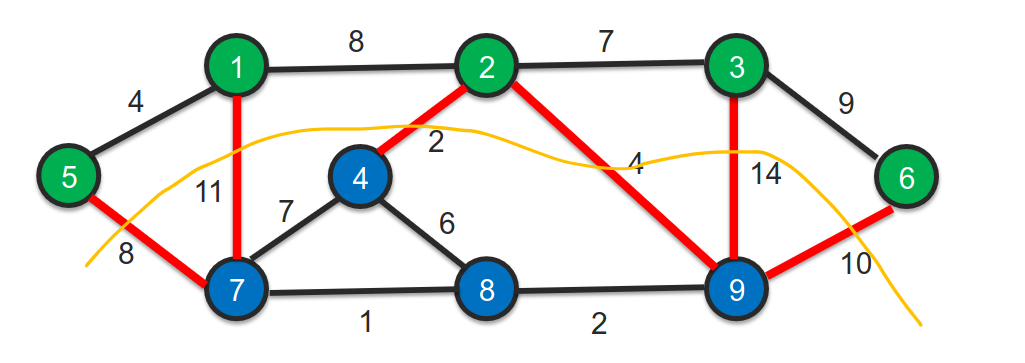
\includegraphics[width=80mm,scale=0.5]{mst_taglio.png}
\end{center}
$V' = \{1,2,3,5,6\}$\\
$V'-V=\{4,7,8,9\}$\\
\subsection{Taglio che rispetta un insieme}
\definizione{Un taglio che \underline{rispetta} un insieme $A \subseteq E$, se nessun arco di A
attraversa il taglio}
\begin{center}
    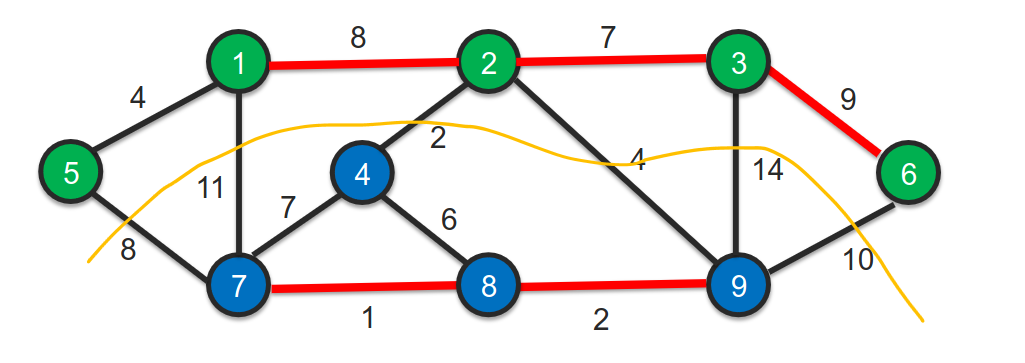
\includegraphics[width=80mm,scale=0.5]{mst_taglio_rispetta.png}
\end{center}
Il taglio rispetta $A = \{(1,2),(2,3),(3,6),(7,8),(8,9)\}$.
\subsection{Arco Leggero}
\definizione{Arco di peso minimo che attraversa il taglio}
\begin{center}
    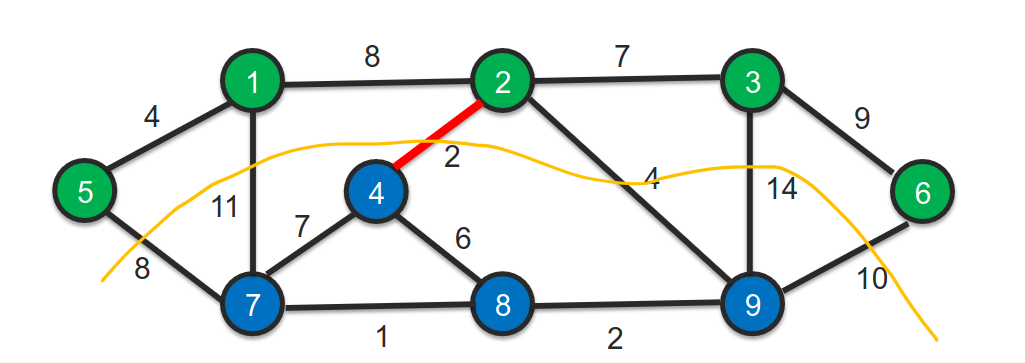
\includegraphics[width=80mm,scale=0.5]{mst_taglio_leggero.png}
\end{center}
(4,2) \ra arco \underline{leggero}
\section{Teorema dell'arco sicuro}
Dati un grafo connesso non orientato e pesato $G=(V,E)$, un sottoinsieme A dell'insieme T di archi di un
Minimum Spanning Tree (MST) e un qualsiasi taglio che rispetti A, allora un arco leggero (u,v) del taglio è
sicuro per A, cioè $A \cup \{(u,v)\} \subseteq T$.
\subsection{Proof}
Considero T \ra insieme di archi di un MST.\\
$A \subseteq T \rt$ sottoinsieme di T.\\
Taglio che rispetta A = (\tikz \fill[green] (0,0) circle (2pt);, \tikz \fill[blue] (0,0) circle (2pt);).\\
$(u,v) \rt$ arco leggero del taglio.
\begin{center}
    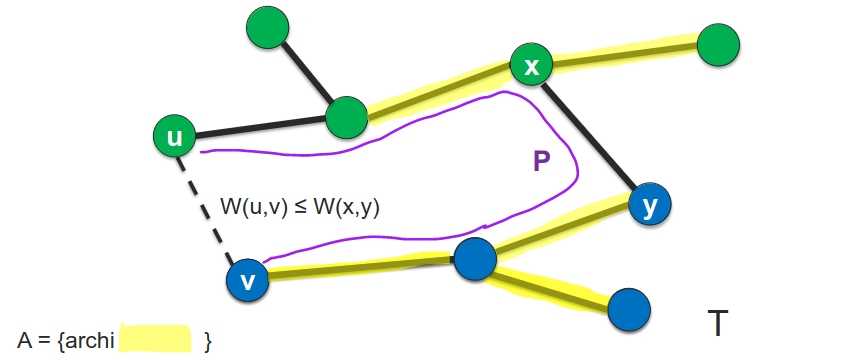
\includegraphics[width=80mm,scale=0.5]{arco_sicuro_dim_mst.png}
\end{center}
Il peso $W(u,v)$ è sicuramente $\leq$ rispetto al peso $W(x,y)$.\\
Sostituisco $(x,y)$, con $(u,v)$ e inserisco quindi l'arco $(u,v)$ all'interno
del grafo e noto che il grafo resta comunque un albero, vedo che resta un MST dato
che non ci sono cicli, ottengo quindi $T'$ con $W(T') \leq W(T)$.\\
\begin{center}
    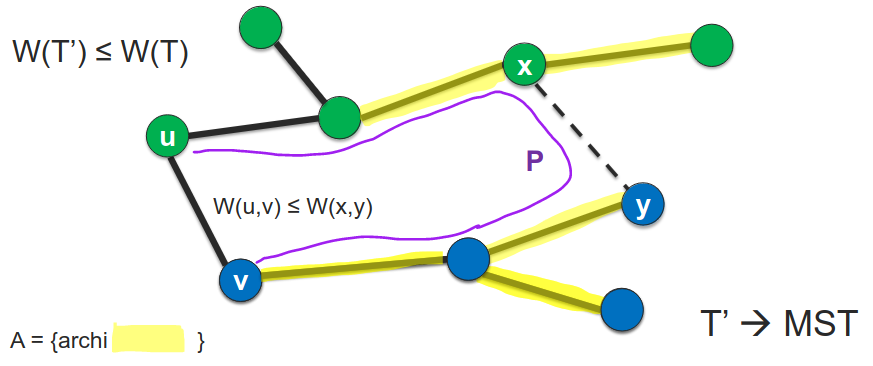
\includegraphics[width=80mm,scale=0.5]{arco_sicuro_dim_mst_2.png}
\end{center}
Per ipotesi, $A \subseteq T$ non contiene $(u,v)$ e $(x,y)$ e per costruzione $T'$ 
non contiene $(x,y)$.\\
$\implies A \subseteq T'$\\
$A \cup \{(u,v)\} \subseteq T'$
\subsection{Esempio Teorema}
Dato il seguente sottoinsieme di T denominato $A = \{archi blu\} \subseteq T$, prendiamo\\
l'arco (2,4) \ra che è arco leggero (dato che ha peso 2), posiamo dire che è un arco sicuro,
infatti se guardiamo T notiamo che $A \cup \{(2,4)\} \subseteq T$, infatti l'arco appartiene
all'MST T.
\begin{center}
    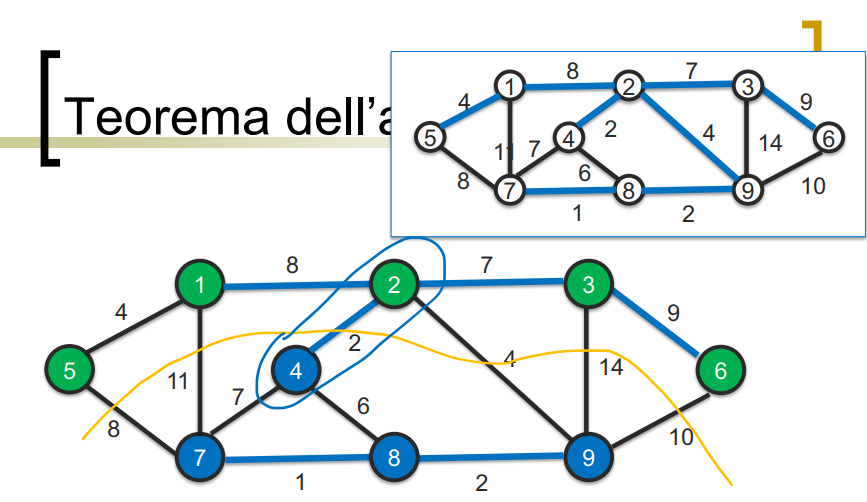
\includegraphics[width=80mm,scale=0.5]{arco_sicuro_es.png}
\end{center}
\subsection{Soluzione generica}
\begin{lstlisting}[language=Java, escapeinside={@*}{*@}]
    Procedura Generic_MST(G,W)
        A = @*\empt*@
        while @*$|V|-|A|>1$*@ do
            trova arco (u,v) sicuro per A
            A = A @*$\cup$*@ {(u,v)}
        return A
\end{lstlisting}
\begin{enumerate}
    \item A rimane aciclico durante le iterazioni
    \item $G_A = (V,A)$ (ad ogni iterazione) è una foresta di $|V|-|A|$ alberi
    \item All'inizio $G_A$ contiene $|V|$ alberti (i singoli vertici)
    \item Ogni iterazione riduce di 1 il numero di alberi e l'arco sicuro (u,v) collega
    sempre componenti distinte di $G_A$
    \item Quando si arriva a un solo albero l'algoritmo termina
    \item Il numero di iterazioni è pari a $|V|-1$
\end{enumerate}
\subsection{COROLLARIO}
$A\subseteq T$ è tale che $G_A = (V,A)$ è una foresta di $|V|-|A|$ alberi.\\
Sia $C= (V_C, A_C), V_C \subseteq V$ e $A_C \subseteq A$, una componente connessa di $G_A$\\
$\implies (V_C, V-V_C)$ è sicuramente un taglio che \underline{rispetta} A\\
$\implies$ un arco leggero di $(V_C, V-V_C)$ è arco \underline{sicuro} per A.\\
\paragraph*{QUINDI} Ad ogni iterazione, per aggiungere ad A un arco sicuro (arco di MST) basta:
\begin{enumerate}
    \item Considerare una delle componenti C della foresta $G_A = (V,A)$
    \item Trovare l'arco di peso minimo che collega un vertice in C con un vertice non in C
\end{enumerate}
\begin{center}
    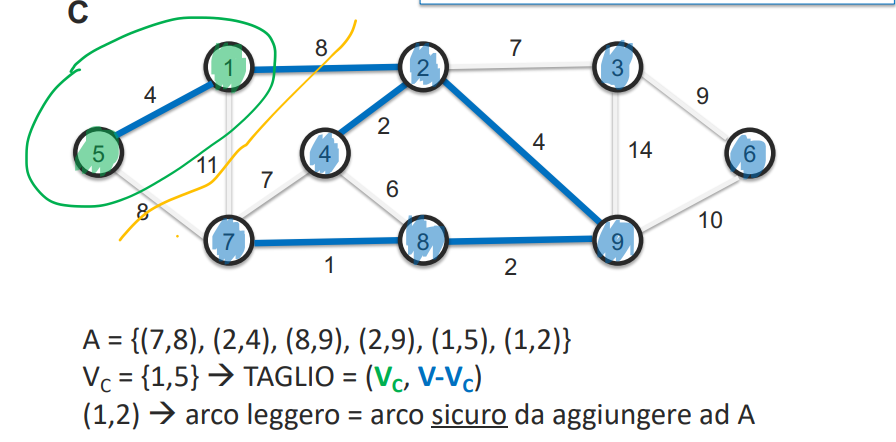
\includegraphics[width=80mm,scale=0.5]{arco_sicuro_corollario.png}
\end{center}
\paragraph*{Corollario} Dati un grafo connesso non orientato e pesato G = (V,E), un
sottoinsieme A degli archi di MST, una componente connessa $C = (V_C, E_C)$ di $G_A = (V,A)$,
allora un arco leggero (u,v) del taglio $(V_C, V-V_C)$ è un arco \underline{sicuro} per A.
\subsection{Implementazione GENERIC-MST}
Ci sono principalmente due implementazioni di GENERIC-MST e sono 2 algoritmi:
\begin{itemize}
    \item Algoritmo di Kruskal
    \item Algoritmo di Prim
\end{itemize}
\section{Algoritmo di Kruskal}
\textbf{MST = Sottoinsieme ottimo di un matroide grafico $M_G$}.
$M_G = (S,F)$ per $G=(V,E,W)$ non orientato e connesso:
\begin{itemize}
    \item S, insieme E degli archi di G
    \item F, tutti i sottoinsiemi di S che sono aciclici
\end{itemize}
pesato con:\\
$W:S \rt R^+$ tale che $W(s)$ è il peso dell'arco s.\\
Sottoinsieme ottimo di $M_G$ pesato con W\\
\ra Archi dello Spanning Tree (ST) di peso massimo.\\
$W':S \rt R^+$ tale che $W'(s) = W_0 - W(s)$\\
$W_0$ è il massimo valore del peso degli archi (massimo per W)\\
Sottoinsieme ottimo di $M_G$ pesato con $W'$\\
\ra Sottoinsieme masimale di peso massimo (per $W'$) e di peso minimo per W che equivale a dire:\\
\ra Archi dello Spanning Tree (ST) di peso \underline{minimo}, cioè l'MST.
\subsection{Algoritmo Greedy Standard per il matroide grafico}.
\begin{lstlisting}[language=Java, escapeinside={@*}{*@}]
    Procedura Generic_matroid_grafic(E = @*$\{e_1, e_2, ..., e_n\}$*@)
        X = @*$\emptyset$*@
        Ordino E per peso W crescente (non decrescente)
        for i form 1 to n do
            if @*$e_i$*@ arco sicuro then
                A = @*$\{e_i\} \cup A $*@
        return A
\end{lstlisting}
\subsection{Algoritmo Kruskal}
\begin{lstlisting}[language=Java, escapeinside={@*}{*@}]
    Procedura KRUSKAL_MST(G = (V,E), W)
        A = @*$\emptyset$*@
        E = @*$\langle e_1, e_2, ..., e_n \rangle$*@ ordinati per peso crescente (non decr.)
        for i form 1 to n do
            if @*$\{e_i\} \cup A \subseteq T$*@ then
                A = @*$\{e_i\} \cup A $*@
        return A
\end{lstlisting}
Devo tradurre in codice l'if che determina se $e_i$ è un arco sicuro e per fare questo
\textbf{applico il corollario}:\\
$e_i = (u,v)$ è arco sicuro se è un arco di peso minimo che connette un vertice di una componente C
con un vertice che non è in C. Quindi $e_i$ è arco sicuro se connette due componenti diverse
di $G_A = (V,A)$. Quindi basta asssegnare l'arco che sto analizzando $e_i$ a $(u,v)$ e se
non appartengono alla stessa componente di $G_A(V,A)$, allora posso aggiungere l'arco alla soluzione A.
\begin{lstlisting}[language=Java, escapeinside={@*}{*@}]
    Procedura KRUSKAL_MST(G = (V,E), W)
        A = @*$\emptyset$*@
        E = @*$\langle e_1, e_2, ..., e_n \rangle$*@ ordinati per peso crescente (non decr.)
        for i form 1 to n do
            (u,v) = @*$e_i$*@
            if u e v @*$\notin$*@ stessa componente di @*$G_A(V,A)$*@ then
                A = @*$\{(u,v)\} \cup A $*@
        return A
\end{lstlisting}
\subsection{Esempio di Esecuzione Algoritmo Kruskal}
\paragraph*{Passo 1} Ordina E per peso non decrescente \ra $E=\langle e_1, e_2, ..., e_m\rangle$,
in modo tale da avere nell'insieme E prima gli archi più leggeri e mano a mano quelli più
pesanti, in questo modo posso applicare un approccio Greedy.\\
Inizializza $A = \emptyset$.\\
\paragraph*{Inizio a considerare gli archi} Considero $e_1 = (7,8)$, connette due componenti di
$G_A$?
\begin{center}
    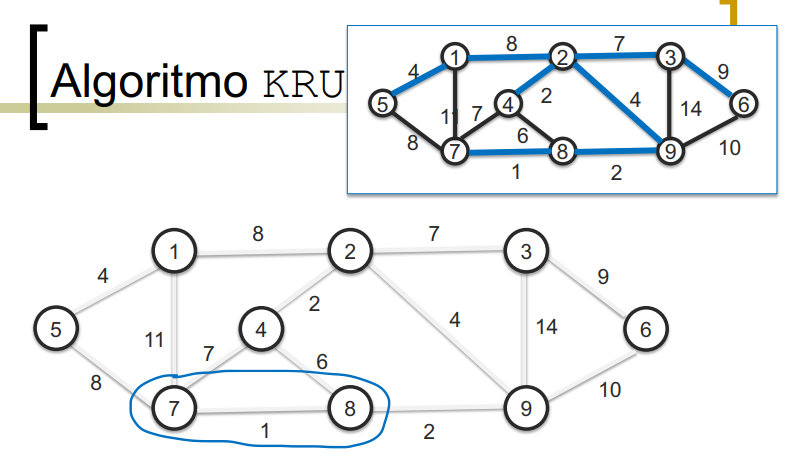
\includegraphics[width=80mm, scale=0.5]{kruskal_esec1.png}
\end{center}
Sì, quindi $\implies A = \{(7,8)\}$.\\
Considero ora il secondo arco $e_2 = (2,4)$, connette due componenti di $G_A$?
\begin{center}
    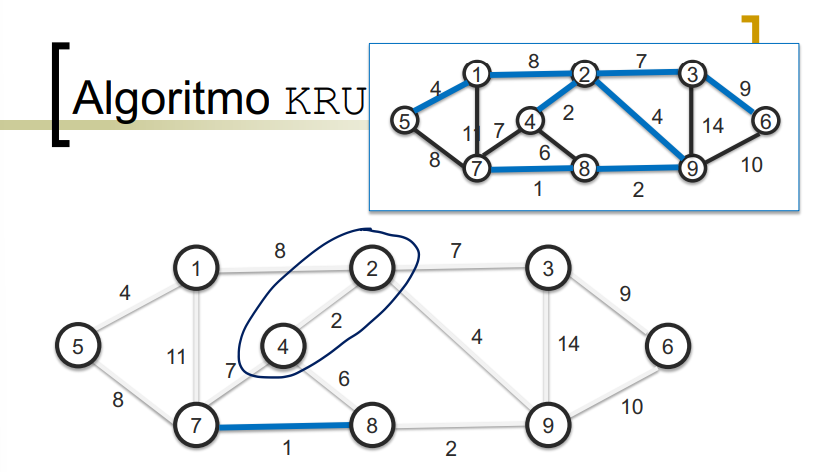
\includegraphics[width=80mm,scale=0.5]{kruskal_esec2.png}
\end{center}
Sì, quindi $\implies A = \{(7,8), (2,4)\}$.\\
Saltiamo qualche passo dove aggiungiamo sempre archi perchè troviamo sempre che
gli archi considerati connettono due componenti.\\
Consideriamo l'arco $e_6=(4,6)$
\begin{center}
    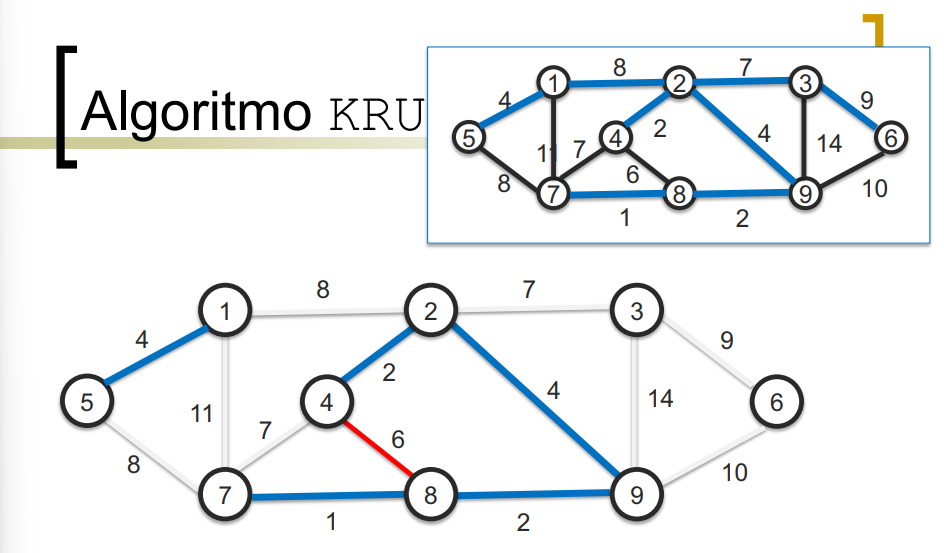
\includegraphics[width=80mm,scale=0.5]{kruskal_esec3.png}
\end{center}
Notiamo che in questo caso l'arco non connette due componenti di $G_A$ (le 
componenti sono già connesse tramite altri archi, aggiungere questo arco creerebbe
un ciclo), per questo non considero questo
arco e procedo a considerare il successivo.\\
Continuo in questo modo fino a quando non ho considerato tutti gli archi. Alla fine
avrò ottenuto l'MST!
\subsection{Codice Kruskal}
Abbiamo già scritto in precedenza il codice di Kruskal, ma come possiamo tradurre le istruzioni
matematiche in codice? Riscriviamo le parti riguardante il controllo di appartenenza al grafo.
\begin{lstlisting}[language=Java, escapeinside={@*}{*@}]
    KRUSKAL-MST(G=(V,E),W)
    A = @*$\emptyset$*@
    E = @*$\langle e_1, e_2, ..., e_n \rangle$*@ ordinati per peso crescente (non decr.)
    foreach v @*$\in$*@ V do
        MAKE_SET(V)
    for 1 from 1 to n do
        (u,v) = @*$e_i$*@
        if FIND_SET(u) @*$\neq$*@ FIND_SET(v) then
            A = @*$\{(u,v)\} \cup A $*@
    return A  
\end{lstlisting}
Tramite la strutture dati FIND SET andiamo ad analizzare se aggiungendo l'arco (u,v), otteniamo
un nuovo albero (quindi connettiamo due componenti) o se abbiamo sempre lo stesso albero (quindi non stiamo
connettendo le componenti, ma stiamo generando un ciclo). se le 2 FIND SET sono diverse allora
possiamo aggiungere l'arco alla soluzione finale tramite la UNION,
altrimenti lo scarto e passo a quello successivo.
\paragraph*{Complessità Algoritmo}
\begin{itemize}
    \item L'ordinamento degli archi avrà complessità $O(|E|\log |E|)$ (Merge Sort)
    \item il MAKE SET avrà complessità $O|V|$
    \item Mentre tutto il blocco for fino a UNION ha complessità $O(|E|\alpha)$, dove
    $\alpha$ è una funzione che cresce molto lentamente che è il tempo di aggiunta degli
    elementi tramite UNION
\end{itemize}
Avendo G connesso \ra $|E| \geq |V|-1$ che possiamo approssimare a $|E|$, quindi
$(|V|+|E|\alpha)$ sarà $(2|E|\alpha)$, ma essendo il 2 un coefficiente costante nell'utilizzo
dell'O è trascurabile.\\
In totale avrò $O(|E|\log |E|+|E|\alpha)$.\\
Sicuramente $\alpha \leq \log |V|$, perchè $\alpha$ cresce molto lentamente
$|V| = |E|$, per questo motivo avrò:\\
\paragraph*{Complessità} $O(E \log|E| + |E|\log |E|)$ quindi\\
$O(|E|\log |E|)$.

\section{Algoritmo di Prim}
Altro algoritmo utilizzato per trovare l'albero di copertura minimo in un grafo che in questo
caso si basa sull'effettuare tagli e scegliere l'arco leggero (quindi sicuro).\\
Si basa sull'assegnazione di un peso ai vertici e questo è un meccanismo utilizzato anche
da un altro algoritmo che vedremo più avanti denominato Dijkstra.
\subsection{Idea dell'algoritmo}
\begin{enumerate}
    \item Sceglie un vertice arbitrario r (componente C iniziale composta dal solo
    vertice r)
    \item Trova l'arco di peso minimo che connette r a un altro vertice v
    (il vertice v entra a far parte di C)
    \item Trova l'arco di peso minimo che connette un vertice in C a un vertice
    v non in C, (il vertice v entra a far parte di C)
    \item Etc.
    \item L'algoritmo termina quando la componente C comprende tutti i vertici
    del grafo e coincide quindi con il Minimum Spanning Tree
\end{enumerate}
\subsection{Proprietà dell'algoritmo}
Ad ogni passo:
\begin{enumerate}
    \item Il sottoinsieme A degli archi di MST aggiunti, stanno tutti nella componente C.
    La foresta $G_A = (V,A)$ è composta da:
    \begin{itemize}
        \item $C = (V_C, A)$
        \item $|V-V_C|$ componenti di vertici singoli
    \end{itemize}
    \item Il taglio $(V_C, V-V_C)$ rispetta l'insieme A
    \item l'arco sicuro è l'arco di peso minimo che connette un vertice in C con
    un vertice non in C
\end{enumerate}
L'idea è quindi quella di effettuare dei tagli tali per cui $(V_C, V-V_C)$ rispetta
l'insieme A, quindi effettuo dei tagli tra l'insieme A gli archi già aggiunti
all'MST e gli altri archi e considero l'arco leggero. Per il teorema dell'arco sicuro, 
l'arco sicuro è l'arco di peso minimo che connette un vertice in C con un vertice
non i C.
\paragraph*{Esempio} Qui di seguito notiamo che effettuando il taglio e scegliendo l'arco
leggero preleviamo automaticamente l'arco sicuro.
\begin{center}
    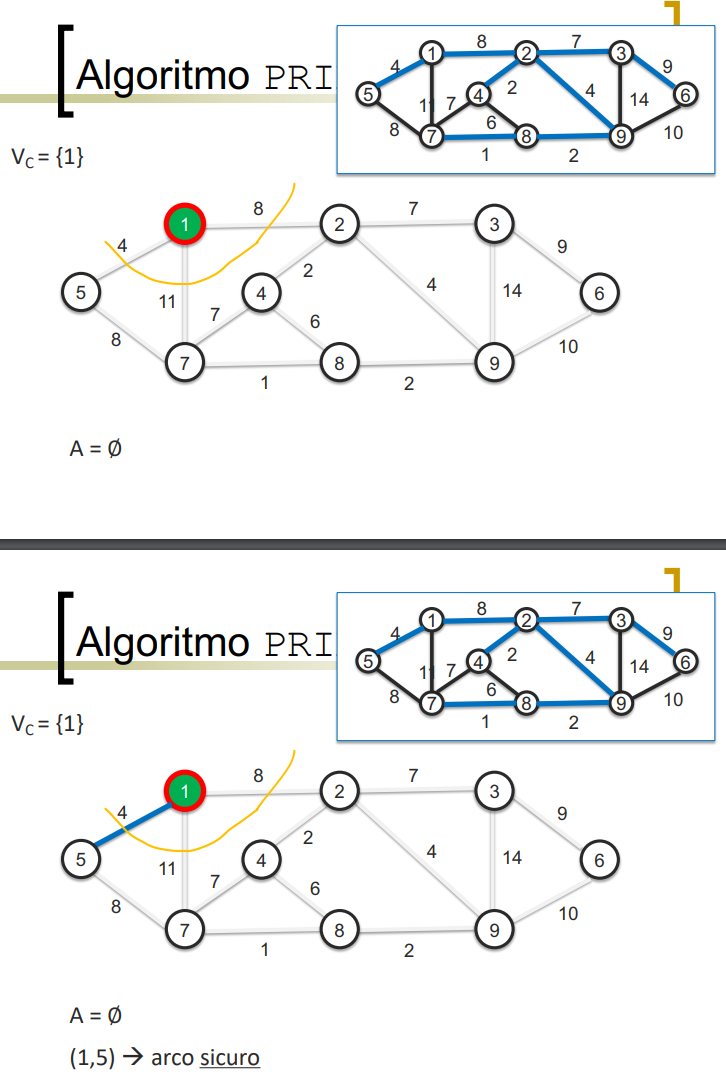
\includegraphics[width=80mm,scale=0.5]{prim_exec1.png}
\end{center}
Continuando ad effettuare tagli validi e a selezione l'arco leggero (quindi sicuro) otteniamo
otterremo l'MST.
\subsection{Implementazione Prim}
Come possiamo implementare in maniera efficiente l'esecuzione del taglio e la
conseguente ricerca dell'arco di peso minimo?\\
Assegneremo dei pesi ai vertici e un valore contenente il suo predecessore per ogni v in V e utilizzeremo
come struttura dati una \textbf{coda Q di min-priority}.\\
La \textbf{min priority queue} è coda particolare che con l'operazione di Dequeue permette
di estrarre l'elemento di priorità minima, in questo caso ci servirà per ottenere sempre l'elemento
di peso minimo.\\
Inizializziamo i pesi a infinito e i valori del predecessore a NIL:
\begin{itemize}
    \item v.key = $\infty$
    \item v.$\pi$ = NIL
\end{itemize}
Scegliamo un vertice r arbitrario, nell'esempio scegliamo $r = 1$ e peso $1.key = 0$.\\
Inseriamo tutti i vertici in una coda Q di min priority che permette l'estrazione 
del vertice con il minimo valore del campo key.
\begin{center}
    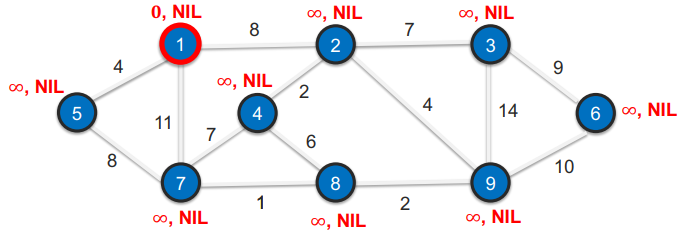
\includegraphics[width=80mm,scale=0.5]{prim_impl1.png}
\end{center}
Estraiamo ora da Q il vertice con il minimo valore di key \ra vertice 1.\\
Procediamo quindi ad esaminare gli adiacenti di 1 \ra 2, 7, 5.\\
2 appartiene a Q and $W(1,2) < 2.key \\ \implies 2.key = (1,2);\quad 2.\pi = 1$.
\begin{center}
    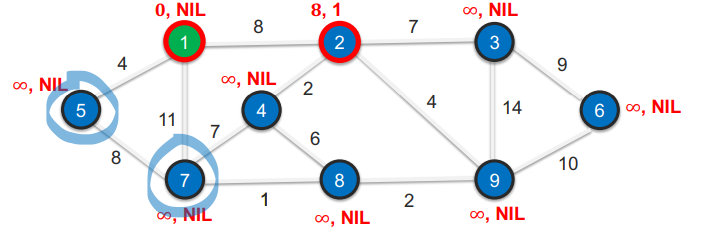
\includegraphics[width=80mm,scale=0.5]{prim_impl2.png}
\end{center}
Considero il secondo adiacente, 7. Esso appartiene a Q and $W(1,7) < 7.key \\
\implies 7.key = W(1,7);\quad 7.\pi = 1$.
\begin{center}
    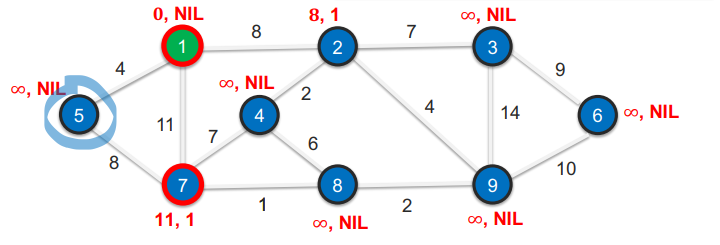
\includegraphics[width=80mm,scale=0.5]{prim_impl3.png}
\end{center}
%slide 236 Continua con l'analisi del terzo vertice adiacente 5
\end{document}